% ---------------------------------------------------------------------------
% simulant — ACS Sensors 판본 Supporting Information (2026-11-02 신설)
%
% 왜 새 파일인가. paper/supplementary.tex 는 elsarticle·JHM 판본이고,
% (1) 표제·저자가 JHM 제목이며 (2) 상호참조가 JHM 본문 라벨을 가리키는데
% 그 라벨 여덟 중 일곱이 ACS 본문에 없었다. 형식만 바꾸면 끊어진 참조가
% 남으므로 파일을 분리하고 참조를 재매핑했다. 재매핑 내역:
%   M-sec:perm    -> M-meth:spaces   (ACS 는 순열검정을 Experimental 에 둔다)
%   M-res:match   -> M-res:panels    (ACS 는 매칭을 2.4 안에서 다룬다)
%   M-meth:panels -> M-meth:spaces
%   M-fig:spaces  -> 대응 도판 없음. 해당 문장을 고쳐 참조를 없앴다.
% 나머지(M-res:panels, M-meth:spaces, M-fig:tox, M-res:docs)는 같은 이름으로
% ACS 본문에 라벨을 달아 그대로 통한다.
%
% journal 코드는 본문과 같은 이유로 jacsat 을 쓴다 (ascefj 는 achemso 목록에
% 없어 절 제목을 삼킨다).
%
% 컴파일: pdflatex -> bibtex -> pdflatex x2. 본문(main)을 먼저 빌드해
% main.aux 가 있어야 xr 상호참조가 풀린다.
% ---------------------------------------------------------------------------
\documentclass[journal=jacsat,manuscript=suppinfo,margin=1in]{achemso}

\usepackage[T1]{fontenc}
\usepackage{amsmath,amssymb}
\usepackage{graphicx,booktabs}
\usepackage{float}
\usepackage{xr}
\externaldocument[M-]{main}
\renewcommand{\arraystretch}{1.15}

% achemso 의 suppinfo 모드는 절에 번호를 매기지 않고(secnumdepth 를 내린다)
% 표·그림 번호에도 S 를 붙이지 않는다. 그 상태에서는 본문의 \ref{S-...} 가
% 빈 문자열로 풀려 "Supporting Information Section sets out ..." 처럼 번호가
% 사라진다 (2026-11-02 렌더에서 확인). ACS SI 관례대로 번호를 되살린다.
% achemso 는 jacsat 에서 절 번호를 끈다 (\SectionNumbersOff). 본문은 그게
% 맞지만 SI 는 'Section S9' 꼴로 가리켜야 하므로 켠다. secnumdepth 만으로는
% 안 된다. 클래스가 \section 자체를 번호 없는 꼴로 바꾸기 때문이다.
\SectionNumbersOn
\renewcommand{\thesection}{S\arabic{section}}
\renewcommand{\thetable}{S\arabic{table}}
\renewcommand{\thefigure}{S\arabic{figure}}

\author{Ku Kang}
\affiliation[CBDRI]{Chemical, Biological, Radiological and Nuclear (CBRN)
Defense Research Institute, Ministry of National Defense, Seoul, Republic of
Korea}
\author{Jeongyun Kim}
\affiliation[CBDRI]{Chemical, Biological, Radiological and Nuclear (CBRN)
Defense Research Institute, Ministry of National Defense, Seoul, Republic of
Korea}
\author{Miae Kim}
\affiliation[CBDRI]{Chemical, Biological, Radiological and Nuclear (CBRN)
Defense Research Institute, Ministry of National Defense, Seoul, Republic of
Korea}
\author{Doo-Hee Lee}
\affiliation[KMA]{Department of Civil Engineering and Environmental Sciences,
Korea Military Academy, Seoul 01805, Republic of Korea}
\author{Jin Yoo}
\affiliation[CBDRI]{Chemical, Biological, Radiological and Nuclear (CBRN)
Defense Research Institute, Ministry of National Defense, Seoul, Republic of
Korea}
\author{Yoon Jeong Jang}
\affiliation[CBDRI]{Chemical, Biological, Radiological and Nuclear (CBRN)
Defense Research Institute, Ministry of National Defense, Seoul, Republic of
Korea}
\email{yjjangchem@korea.kr}

% achemso 의 suppinfo 모드가 제목 앞에 'Supporting Information:' 를 스스로
% 붙인다. 제목에 또 쓰면 두 번 찍힌다 (2026-11-02 렌더에서 확인).
% 2026-11-03. 본문 제목 교체에 맞춰 동기화.
\title{No Resolvable Agreement Between Descriptor Distance and Colorimetric
Array Response: A Reanalysis of Authentic Chemical Warfare Agent Measurements}

\begin{document}

\maketitle

\noindent This Supporting Information carries the acute toxicity axis, the
predictive interpolation of that axis, the decoupling test between fidelity
and toxicity, the phosphorus-local reactivity analysis, the full permutation
family with every multiplicity scheme, and the controls on dimensionality,
subspace choice and descriptor-block weighting. These results stand on their
own data and are referenced from the main text where they bear on it. They
are placed here because the argument of the main text turns on the
composition of the comparison panel and on whether descriptor distance
predicts measured array response, and does not depend on them.

\section{Safety axis}
\label{meth:aegl}
Acute inhalation toxicity was taken as the EPA AEGL-3 value at 10~min,
the concentration above which life-threatening effects or death are predicted,
parsed directly from the official compiled table \cite{epaaegl2018}; the
derivation of these values for the agents is described by
Watson et al.~\cite{watson2006}, and the concentration--time exponent on which short-exposure
extrapolation of such criteria rests was established by ten Berge et al.~\cite{tenberge1986}.
A single fixed exposure duration was used rather than a derived
concentration--time surface, and the tier value is used directly as a
per-compound property rather than as an exceedance probability. Agent
degradation products, which carry their own and in places
distinct toxicity \cite{munro1999}, are outside the compound set. Values
published in ppm were converted using
$c\,[\mathrm{mg\,m^{-3}}] = c\,[\mathrm{ppm}] \times M / 24.45$. Compounds
without a value are recorded as such, with the reason, and are never imputed.

Extraction is the step on which every safety-axis number depends, so we describe
it in full. The compiled table carries 270 chemical entries that present an AEGL
table of their own, besides a holding list of substances for which the agency
states that values are not being developed. Reading a
ten-minute AEGL-3 from one of them is not simply a matter of taking the first
number on the AEGL-3 line, for four reasons that the table itself imposes. Some
entries place a footnote marker in the ten-minute cell and give the value below
the table, as \textit{AEGL 3 - 10 min = ** 40,000 ppm}, because the value exceeds
half the lower explosive limit. Some give values only for the shorter durations
and \textit{NR} for the longer ones, so the row carries three numbers rather than
five. Some print the agency's own mg~m$^{-3}$ equivalent beside each value, in
brackets for the agents and in parentheses elsewhere. And the text layer of the
document occasionally breaks one row across two lines. We therefore parse each
AEGL row into exactly five duration cells, where a cell is a number, an
\textit{NR}, a \textit{see below}, or a bare footnote marker, and refuse to use
any row that does not yield five; footnote lines are separated from table rows by
grammar before parsing, and the ten-minute value is read from the text following
the footnote's equals sign, so the duration labels that precede it cannot be
mistaken for values. Of the 270 entries, 261 yield a ten-minute AEGL-3: 252 from a table cell and
nine from a footnote. Two of those 261, magnesium aluminium phosphide and a 60\%
nonafluoroisobutyl ether preparation, carry no registry number in the table and
are set aside here, because without one their structure cannot be resolved
unambiguously, which leaves 259 (250 from a table cell and nine from a
footnote). They are not the two set aside in Section~\ref{sec:qsar}, which have
registry numbers but no single molecular structure.

Two independent checks were applied, and the distinction between them matters.
The conversion constant was checked against the agency's own bracketed
mg~m$^{-3}$ figures, which it reproduces to within 0.9--4.0\% over eight
comparisons (GB, GD, GA and GF at AEGL-2 and AEGL-3). That check validates the
arithmetic and nothing else: every agent value carrying a bracketed conversion is
below 1~ppm and contains no thousands separator, so a defect in numeric
extraction could not appear in it. The extraction itself was therefore checked
over the whole table by a second reader that shares neither the text-extraction
engine nor the algorithm: it renders the document with a different tool, locates
the character columns of the five duration labels in each header line, and reads
the ten-minute value from the corresponding substring of the AEGL-3 line. A
positional reader of this kind cannot reproduce a token-ordering fault, which is
the point of using one. The two readers agree on all 250 entries for which both
read a value from a table cell, on all 257 of
those that resolved to a structure and on all nineteen values in the
twenty-eight-compound panel. They do not agree on how many entries the table
holds: the positional reader opens 269 where the primary reader opens 270, a
difference of one entry that it declines to open rather than reads differently.
Agreement on every compared value is therefore agreement over the 250 the two
readers both reach, not over the whole table, and we state the coverage because
the distinction is the one this check exists to make. Thirty-four values reach 1000 or more, where a
thousands separator appears; twenty-five are read from a table cell and nine
from a footnote, and 33 of the 34 are covered by the comparison against the
training set. We report the coverage of this check
and not only its pass rate, because a validation sample that excludes the failure
mode it is meant to detect establishes nothing. An earlier version of this check
compared in one direction only, over the entries that reached the training set,
and restricted the thousands-separator count to the table-cell path. Both
restrictions removed the failure mode from the sample: the positional reader
carried one record-boundary fault, assigning a neighbouring compound's value to
ricin, and ricin does not resolve to a structure, so no one-directional
comparison could have seen it. The fault is corrected, the comparison is now
made in both directions, and the count covers both paths.

\section{Predictive interpolation of the safety axis}
\label{sec:qsar}
To test whether the missing values could be filled, a random forest was trained
on $\log_{10}$(AEGL-3, 10~min) using 37 RDKit descriptors, with five random seeds,
five-fold cross-validation and 10\,000 bootstrap resamples for interval
estimates. Of the 259 entries with a ten-minute AEGL-3, 257 resolved to a
structure through PubChem; the two that did not are a mixed-isomer entry and a
protein toxin, neither of which has a single molecular structure. Five of the 257
are interhalogen compounds that RDKit cannot parse, and two were removed because
their stored structure failed the identity check described below, leaving 250.
Twenty of these are military chemical agents, identified by registry number
rather than by matching on name, and all twenty were held out of training and
used only for evaluation, leaving 230 for training. The held-out set is the G
series including cyclosarin, VX, sulfur mustard, the three nitrogen mustards,
lewisite~1, methyldichloroarsine, ethyldichloroarsine, phenyldichloroarsine,
diphenylchloroarsine, adamsite, BZ, phosgene oxime, hydrogen cyanide, phosgene
and chloropicrin. Matching on names rather than registry numbers is what makes
such a set hard to assemble: the table lists cyclosarin as ``GF Agent'', which a
pattern written for ``Agent G'' does not find, and it lists three arsenical
vesicants and BZ in rows whose longer durations are \textit{NR}, which a parser
that requires five numbers per row discards entirely. External validation on
held-out compounds rather than cross-validated statistics
alone is the minimum standard for a predictive structure--activity model
\cite{gramatica2007,tropsha2010}. An applicability domain was defined as the
mean distance to the five nearest training compounds in standardised descriptor
space, with the boundary at the 95th percentile of the training set's own such
distances. This is the $k$-nearest-neighbour distance criterion whose relation to
prediction accuracy was established by Sheridan et al.~\cite{sheridan2004} and which appears
among the standard formulations surveyed by Netzeva et al.~\cite{netzeva2005} and
Roy et al.~\cite{roy2015}; we have used the same construction to bound predictions in
hazard-prioritisation screens \cite{dbpcarto}. Whether such a domain can detect
a compound that is close in descriptor space but outside the training set's
mechanistic coverage is precisely what Section~\ref{res:qsar} tests, and is
related to the open-set problem of recognising an input as unfamiliar rather than
assigning it to a known class \cite{openset}.

\section{Decoupling test}
Candidates were the AEGL compounds for which structure, electronic descriptors
and a measured AEGL-3 were all available, excluding the authentic agents
themselves ($n=207$). Eight further records were set aside under four rules
declared in advance, all of which ask the same question: are these electronic
descriptors defined for that species at all? A record is excluded if
its stored structure has more than one component, because the relative placement
of the fragments is arbitrary and the dipole moment is therefore undefined
(three records); if the species is open-shell, because the orbital parse reads
only one spin manifold, so that its HOMO and LUMO do not carry the
closed-shell meaning (three); if it is a bare atom with no
bonds, because molecular descriptors carry no meaning (three); or if the
HOMO--LUMO gap is below 0.5~eV, because a closed-shell single-reference
description does not hold at that gap and the orbital energies themselves stop
meaning anything (one). Some records fall under more than one
rule. The gap rule bites on a single record: sodium cyanide returns
a gap of 0.097~eV where the next smallest gap in the pool is 1.31~eV, so the
0.5~eV bar separates that one record and no other. Retaining all eight
records raises the candidate count to 215 and moves the Spearman coefficient
from $+0.062$ to $+0.030$, leaving
every conclusion in Section~\ref{res:h1} unchanged. Fidelity was defined as the standardised
Euclidean distance in the three-coordinate electronic space to the nearest
authentic agent; safety as the measured $\log_{10}$(AEGL-3). For the quadrant analysis, the safety bar
was set at the measured AEGL-3 of dichloromethane, the incumbent
simulant, read from the parsed table rather than entered by hand; a replacement
simulant should not be more acutely toxic than the compound it replaces. Because
that bar turns out to be demanding, the count is also reported at one and two
orders of magnitude below it. Association was tested with Spearman and
Pearson correlation, with 10\,000-resample bootstrap confidence intervals
\cite{efron1986}. Effect sizes are reported with intervals rather than
$p$-values alone \cite{nakagawa2007}. Where a paired comparison was made,
normality of the paired differences was assessed by the Shapiro--Wilk test
\cite{shapiro1965} and the Wilcoxon signed-rank test \cite{wilcoxon1945} used
in place of a paired $t$-test where normality was rejected; those paired tests
are reported for completeness only, because, as Section~\ref{M-meth:spaces} explains,
they are confounded by group size and the exact permutation test supersedes them.
\section{Conformer dependence of the shape descriptors}
\label{meth:conformer}

Nine of the coordinates in every structural space are read from a
three-dimensional structure rather than from the SMILES string, so they depend
on which conformer the descriptor build uses. The first version of this work
took the single lowest-energy member of an ETKDGv3 ensemble of at most twenty,
pruned at 0.5~\AA{} RMSD. That choice was never stated, and it did not
reproduce: rebuilding the cache from the deposited code returned eleven of
fifty-two numeric columns different from the deposited values, the worst by 72
per cent of its own magnitude. The cause is that the selection is an
\texttt{argmin} over near-degenerate force-field energies, so a small numerical
difference between runs moves it to a different conformer.

We therefore replaced the selection with a Boltzmann-weighted mean over the
whole ensemble at 298~K. Every numeric column of the cache now reproduces from
the code. The descriptor build script checks this under a
\texttt{--verify} flag, and the analysis pipeline requires it before it will
run.

The seed moves one of the eleven agents and nothing else. Repeating the
embedding under six seeds and rebuilding only the nine shape coordinates, the
thirty-five-compound panel returns no valid match in any of the twelve runs and
the retained merged space is thirty-eight coordinates in all twelve. On the
twenty-eight-compound panel the count is three under all six single-conformer
seeds, and three under three of the six ensemble seeds against four under the
other three. The agent that moves is tabun in every case. Its normalised
distance runs from 1.9943 to 2.0106 across the ensemble seeds and from 2.0172 to
2.0273 across the single-conformer seeds, against a threshold of 2, so the whole
spread lies within 0.03 of the threshold and straddles it. The merged-space
permutation value runs from 0.0250 to 0.0279 under both treatments. Values are
in the two deposited files
\texttt{conformer\_sensitivity\_ensemble.json} and
\texttt{conformer\_sensitivity\_single.json} under \texttt{outputs/}.

We report this at length because the conformer is a choice of the same kind as
the panel, the space and the statistic, and we had not counted it. It belongs in
the list of Section~\ref{M-res:panels}, and unlike the other four it does not
change what the panel says about any agent except tabun. What it establishes
about tabun is that this analysis does not determine whether tabun has a valid
match. The embedding seed decides it, and so does the order in which the
correlation filter is handed its columns
(Section~\ref{meth:orderinvariance}). We report tabun as a borderline case
throughout rather than counting it on either side.

\section{Column order in the correlation filter}
\label{meth:orderinvariance}

The descriptor spaces are built by dropping one coordinate from every pair whose
absolute Pearson correlation exceeds 0.95, so that no retained pair sits above
that cut. More than one retained set satisfies that constraint, and until this
revision the set we used was chosen by the order in which the columns happened
to sit in the descriptor file. The filter walked the pairs in that order and
dropped the later member of each supra-threshold pair, which means the surviving
coordinates were a function of a variable no analyst had selected.

The cost is measurable. Permuting the input column order forty times under a
fixed seed and rebuilding everything downstream, the old filter returned
thirty-seven distinct retained sets on the twenty-eight-compound panel, with
dimensions between 36 and 39, and a valid-match count of three in twenty-five
of the forty orderings and four in the remaining fifteen. The value we had
reported was the minority outcome. The thirty-five-compound panel behaved
differently: thirty-six distinct retained sets and dimensions between 39 and 41,
but a valid-match count of zero in all forty orderings. The headline negative
result on the primary panel never depended on column order; the positive count
on the reduced panel did.

One concrete case shows how the old filter reached a set it should not have. It
dropped \texttt{chi0v} against molecular weight at $|r| = 0.9532$, which removed
the only partner \texttt{kappa1} had above the cut, so \texttt{kappa1} survived
even though $|r|(\texttt{kappa1}, \texttt{chi0v}) = 0.9816$. The retained set
therefore contained a coordinate correlated at 0.98 with one the filter had just
discarded as redundant.

We replaced the rule rather than fixing the order. The filter now follows the
\texttt{findCorrelation} rule of Kuhn\cite{caretref}: take the pair with the
largest $|r|$, drop whichever of its two members has the larger mean $|r|$
against the other retained coordinates, recompute the correlation matrix, and
repeat until no pair exceeds the cut. Three conventions make it deterministic.
The input columns are sorted by name before the first pair is examined, so the
caller's order cannot matter. Where exactly one member of a pair is a protected
coordinate, the unprotected one is dropped, which takes precedence over the mean
correlation and was a rule in the previous filter as well. Where the two mean
correlations agree to within $10^{-12}$, the later name in lexicographic order
is dropped, a path reached only by exactly duplicated columns.

Under the new rule the same forty permutations return a single retained set on
every panel: thirty-eight coordinates and three valid matches on the
twenty-eight-compound panel, forty-one coordinates and no valid match on the
thirty-five-compound panel, and forty-one coordinates with five valid matches
when the five literature-proposed simulants are admitted alongside the three
incumbents, eight candidates in all. The maximum
retained $|r|$ is 0.9470, as it was before. The counts are in
\texttt{order\_invariance.json} under \texttt{outputs/} and are regenerated by
\texttt{order\_invariance.py}, which reports both rules side by side.

The agent that moves between the two rules is tabun, and it moves because its
normalised distance to dimethyl methylphosphonate crosses the threshold of 2:
1.9948 under the old filter against 2.0038 under the new one. Section
\ref{meth:conformer} shows the conformer embedding seed moving the same quantity
across the same threshold. Taken together, tabun's normalised distance lies
within 0.03 of the threshold under every treatment we have run, and whether it
counts as a valid match is decided by implementation choices rather than by the
data. We therefore report three valid matches on the twenty-eight-compound panel
and name tabun as a borderline case wherever the count appears, rather than
presenting either three or four as settled.

\section{Sparse indicator columns and the distance they add}
\label{meth:sparse}

Eleven of the thirty-eight retained coordinates of the merged space are binary,
and they are not evenly populated. Four are carried by exactly one compound of
the twenty-eight: \texttt{n\_As} by lewisite~1, \texttt{n\_P\_CN} by tabun,
\texttt{n\_P\_S} by VX and \texttt{n\_nitro} by chloropicrin. One is carried by
two compounds, three by three, two by four and one by five.

A binary column with a single one has mean $1/n$ and sample variance exactly
$1/n$, so its standard deviation is $n^{-1/2}$ and standardising it places the
carrier and every non-carrier exactly $\sqrt{n}$ apart. The squared Euclidean
distance between the carrier and every other compound therefore gains exactly
$n$, which is 28 here, from that one column, while the distance between two
non-carriers gains nothing. We verified the figure against the standardised
column rather than relying on the algebra; it is 28.000000.

What that addition encodes is that the compound is the only one of its kind in
this panel. It is a true statement about the panel and it carries no information
about proximity to any particular simulant, yet it enters the distance on the
same footing as molar refractivity. The effect is concentrated on four
agent-to-simulant distances. For tabun against DMMP the four single-carrier
columns are 47.6\% of the squared distance, essentially all of it from
\texttt{n\_P\_CN}; for VX against dipropylene glycol monomethyl ether 20.4\%;
for lewisite against dichloromethane 41.8\%. For sarin, soman and cyclosarin,
which carry none of the four, it is zero. Counting all eleven binary columns
rather than the four raises tabun's share to 72.1\% and sarin's to 48.8\%.

\begin{table}[htb]
  \centering
  \caption{Valid matches on the twenty-eight-compound panel as sparse indicator
  columns are removed. The threshold for a binary column is the number of
  compounds carrying a one. The last row removes every coordinate with five or
  fewer distinct values, which also removes two counts and one protected
  coordinate and is the least defensible of the variants. The one-sided $p$ is
  the merged-space exact enumeration over all $\binom{17}{3}=680$ designations.}
  \label{tab:sparse}
  % 2026-11-03. outputs/tab_sparse.tex 로 자동 생성.
% 자동 생성 — make_si_tables.py. 손으로 고치지 말 것.
  \begin{tabular}{lrrrrr}
    \hline
    Encoding & Removed & Dim. & Matches & Tabun $d_{\mathrm{norm}}$ & $p$ \\
    \hline
    As reported                  &  0 & 38 & 3 & 2.0038 & 0.0250 \\
    Drop single-carrier binaries &  4 & 34 & 4 & 1.4509 & 0.0250 \\
    Drop binaries with $\le 2$   &  5 & 33 & 4 & 1.4509 & 0.0206 \\
    Drop binaries with $\le 3$   &  8 & 30 & 5 & 1.6780 & 0.0162 \\
    Drop binaries with $\le 4$   & 10 & 28 & 4 & 1.4392 & 0.0132 \\
    Drop binaries with $\le 5$   & 11 & 27 & 4 & 1.2455 & 0.0132 \\
    Drop cardinality $\le 5$     & 14 & 24 & 6 & 1.1604 & 0.0074 \\
    \hline
  \end{tabular}

\end{table}

Table~\ref{tab:sparse} gives the sweep. Every removal raises the count above
the three of the reported encoding and lowers the nominal $p$, though the count
is not monotone in how much is removed: it reaches five at one setting and
returns to four at the next. The
encoding we report is the one that produces the fewest matches and the largest
$p$ of the seven. We state that plainly because it is the only evidence
available that the encoding was not selected for its answer, and because a
reader who repeats this analysis with a different descriptor set will get a
different count.

The agreement test between descriptor distance and measured response does not
behave this way. Recomputing the twelve Mantel tests of
Section~\ref{M-res:mantel} under the first, second and fourth encodings of
Table~\ref{tab:sparse} leaves the smallest Benjamini--Hochberg value at 0.1167,
0.4722 and 0.3889 respectively, with no cell below 0.05 under any of them.
Removing the single-carrier indicators makes the agreement weaker, not
stronger. The paper's result is in that test, and it is the one quantity here
that no analyst choice we enumerated has moved.

\section{Lewisite purity and what depends on it}
\label{meth:purity}

The second run reports GC--MS purities above 95\% for hydrogen cyanide,
cyanogen chloride, phosgene, chloropicrin, sulfur mustard and nitrogen
mustard, and 67\% for lewisite~1.\cite{multiplexref} The first and third runs
report no purity values; we searched the methods of both and found none, and we
do not estimate them.

A 67\% sample is a mixture, and lewisite enters both the descriptor panels, as
one of the eleven agents, and the second run's premise test, as one of seven
compounds. Removing it changes neither. On the twenty-eight-compound panel the
count stays at three valid matches with the dimension falling from 38 to 37; on
the primary panel it stays at zero with the dimension falling from 41 to 39;
admitting the five literature-proposed simulants, eight candidates in all, it
stays at five. In the second run's
premise test the mean difference moves from $+0.558$ to $+0.529$ in the
ultraviolet channel and from $+0.619$ to $+0.625$ in reflectance. The
sign-flip $p$ recorded at the time rose from 0.0078 to 0.0156 in both, which
is that test's design floor moving with the compound count from $2^{-7}$ to
$2^{-6}$ and carries no information. We withdraw the sign-flip test in
Section~\ref{meth:deltaE}, and this sensitivity does not rest on it: the
statistic itself moves by 0.029 and 0.006, so removing lewisite does not
change what either cell shows. The counts are in \texttt{purity\_sensitivity.json} under
\texttt{outputs/}.

\section{Density-functional check on the electrophilicity axis}
\label{meth:dft}

The electronic descriptors throughout this work are GFN2-xTB. That method is
parameterised for geometries and energies rather than for virtual orbital
energies, so any quantity built from its LUMO carries a question we cannot
answer from inside the method. We therefore recomputed the frontier orbital
energies of all twenty-eight compounds of the smaller panel at
B3LYP/def2-SVPD, a basis chosen because it carries diffuse functions, which
virtual orbitals need, and covers arsenic, which lewisite needs. From those we
formed $\mu$, $\eta$ and $\omega = \mu^{2}/2\eta$ by the same definitions used
throughout. The same converged calculations also give the dipole moment, which
the third paragraph of this section uses.

The comparison is not clean, and we say so rather than letting it read as one.
The GFN2 values in this paper sit on GFN2-optimised geometries, which we could
not reproduce in the environment where the check was run; the density-functional
values sit on RDKit ETKDG geometries relaxed with MMFF94, or with UFF for
lewisite, whose arsenic MMFF does not parameterise. The difference between the
two sets of $\omega$ therefore contains a geometry term as well as a method
term, and we do not attempt to separate them. What the check can establish is
whether an ordering drawn from the GFN2 $\omega$ axis is stable, and it is not
(Section~\ref{res:plocal}). What it cannot establish is the size of the method
term alone. All twenty-eight calculations converged; values are in the deposited
\texttt{outputs/dft\_omega.csv}. The dipole moments were obtained in a second
pass over the same twenty-eight molecules, which reproduced both orbital
energies of every compound to within $10^{-6}$~eV before the dipoles were read;
that pass is deposited separately as \texttt{outputs/dft\_dipole.csv} so the
reproduction can be checked rather than taken on assertion.

% 2026-11-02 (GATE 8 7차). 이 절이 쌍극자 재계산을 설명하면서 두 방법의
% 일치도를 한 번도 수치로 내놓지 않았다. 가장 큰 편차가 이 논문의 주인공
% 화합물에서 난다는 사실이 특히 보고되어야 한다.
The two sets of dipole moments agree at a Pearson $r$ of 0.9195 over the
twenty-eight compounds, with a mean absolute difference of 0.328~D. The
agreement is not uniform, and the largest single disagreement falls on the
compound this paper is most concerned with. DMMP is 2.523~D under GFN2 and
4.883~D under the density functional, a difference of 2.359~D, which is
almost the size of the semiempirical value itself. Lewisite follows at
0.795~D against 2.108~D, consistent with the arsenic trichloride case noted
below and with the force field used for that molecule, which is UFF because
MMFF does not parameterise arsenic. Sarin is third at 3.640~D against
4.286~D. No other compound differs by more than 0.52~D. A reader weighing
the electronic-space result of Section~\ref{M-res:panels} should know that
the coordinate most likely to move under a change of method is the one on
which DMMP sits furthest from where the semiempirical method places it.

The same recomputation answers a second question, and we report the answer
although it does not favour the analysis. The electronic space that carries the
results of Section~\ref{res:permfull} has three coordinates: the two frontier
orbital energies this check has just recomputed, and the dipole moment. The
dipole follows from the same converged self-consistent field at no further cost,
so there is no reason to leave it semiempirical, and we took all three
coordinates from the density functional. We then repeated the matching rule of
Section~\ref{M-res:panels} and the exact permutation over all 680 designations.
The control reproduces what the main text reports, one valid match of eleven and
a one-sided $p$ of 0.275. Replacing the two orbital energies and leaving the
dipole at GFN2 gives four valid matches and 0.128. Replacing all three gives
five valid matches and 0.0368. Four of those five are sarin, soman and tabun
matched to DMMP and cyclosarin matched to DPGME, pairings the designation record
supports. The fifth is sulfur mustard matched to DPGME, about
which the designation record says nothing either way: the patent that names
DPGME requires detectability by ion mobility spectrometry of the composition
and assigns the compound to no agent class (Section~\ref{M-res:docs}). An
earlier version of this section wrote that the patent calls DPGME a preferred
G-agent simulant and rejected this pairing on that ground. We withdraw that
statement because we could not verify the wording against the patent
itself. The single match under GFN2 was hydrogen cyanide to
dichloromethane.

Three things have to be said about that. The first is that the sign of the
conclusion in this one space depends on the electronic-structure method. Under
GFN2 the electronic space was where the incumbents did worst and nothing in it
came near significance; under the density functional the same space, the same
matching rule and the same exact permutation return 0.0368. We do not promote
that value to a positive finding. It is a single uncorrected statistic in one
space, reached by changing a method after seeing the first answer, and the
geometry confound of the preceding paragraph applies to it in full. We report it
because the alternative is to leave standing a negative claim that our own check
does not support. The second is that the merged space does not move the same
way. Rebuilt from the same three density-functional coordinates it retains the
thirty-eight coordinates of the main analysis and returns three valid matches and
a one-sided $p$ of 0.0250, against four and 0.0250 for the GFN2 control, so the
value the main text carries is not an artefact of the semiempirical method. The
third is that the analyst freedoms this paper is about therefore include one we
did not enumerate when we set the comparison up, and it is the freedom that
moved the electronic space furthest of any we examined. Values are in the
deposited \texttt{outputs/dft\_electronic\_space.json}.

We did not extend the check to the condensed Fukui index. The only population
scheme available to us at this level is a Mulliken partition, and on a diffuse
basis that can return a negative condensed index for electrophilic attack, which
is an artefact of the partition rather than a chemical statement. We therefore
have no independent check of this quantity. The
$f^{+}(\mathrm{P})$ values in Table~\ref{tab:plocal} are therefore GFN2 values
with no independent check, and the ratio between DMMP and VX that the main text
quotes should be read within that limit.

\section{Multiplicity and the accounting schemes}
\label{meth:multiplicity}
Multiplicity is corrected within each panel configuration. The six distance
statistics applied to the three descriptor spaces form one family of eighteen
tests on the same descriptor table, and we report the whole family rather than a
selection from it, so the Benjamini-Hochberg procedure \cite{benjamini1995} is
applied across those eighteen and the smallest adjusted value is given in
Table~\ref{tab:ablation}. An earlier version of this work reported one nominal
value per space and declined to correct, on the ground that the spaces were
separate analyses. That ground fails once the statistic is also chosen by the
analyst, and we treat the earlier position as an error rather than a convention.

Defining that family is itself a choice, and a paper arguing that such choices
decide the answer cannot leave its own unexamined. We therefore report four
schemes rather than one. The eighteen tests are corrected together; the six
statistics are corrected within each space separately, treating the spaces as
three analyses; a single statistic, the mean difference, is treated as though it
had been specified in advance, leaving three tests; and, because the three
spaces are nested and the six statistics are functions of one distance matrix,
the dependence is handled exactly rather than approximated. All eighteen tests
are computed on the same enumeration of designations, so the joint null
distribution is available: for each designation we convert every test statistic
to its one-sided $p$ within its own null, take the smallest of the eighteen, and
read the observed smallest $p$ against that distribution. This is the
single-step min-$P$ procedure of Westfall and Young \cite{westfall1993}, and
because the permutations are shared it requires no assumption about the
correlation structure. We also report the approximation it replaces, the
effective number of independent tests estimated from the eigenvalues of the
correlation matrix of the eighteen nulls by the method of Li and Ji
\cite{liji2005} used as a Bonferroni divisor, so that the two can be compared.
The five answers are given in Table~\ref{tab:family} and they do not agree.

\section{Dimensionality and subspace controls}
\label{meth:dimdetail}
The structural and electronic spaces differ in dimension by more than an order of
magnitude, and the concentration of Euclidean distances depends on dimension, so
a difference between the two spaces is not by itself a difference between
chemistries. We bounded the effect in two ways, both reported in
Section~\ref{res:dimdetail}. The standardised structural space was truncated to its
first three principal components and the permutation test rerun on that
three-dimensional space. Separately, 2000 random three-descriptor subsets of the
structural space were drawn without replacement (seed \texttt{0xC0DE}) and the
full exact permutation test run on each, giving the distribution of $p$ that an
arbitrary three-dimensional slice of these descriptors produces. The observed
structural value is interpretable only against that distribution.

The random-subspace control of Section~\ref{meth:dimdetail} draws three descriptors
from a correlated pool, so three descriptors do not carry three degrees of
freedom and the resulting rate of nominal significance may be inflated. We
repeated it on ZCA-whitened coordinates, obtained by standardising the
structural block, taking the eigendecomposition of its covariance, and applying
$V\Lambda^{-1/2}V^{\top}$ over the non-null eigenvalues, so that the coordinates
drawn from are uncorrelated by construction. Both the raw and the whitened rates
are reported. That draw count carries a Monte Carlo
standard error near one percentage point on a proportion and resolves a
percentile to 0.05.

\section{Measured colorimetric array response}
\label{meth:deltaE}
Measured response was taken from a 29-dye colorimetric array reported in earlier
work from this laboratory \cite{hazref,multiplexref,group3ref}. Colour difference
$\Delta E$ is the CIEDE2000 difference against the zero-concentration image of
the same dye in the same channel, given per dye for three compound sets at
solution concentrations of 10, 50, 100 and 500~$\mu$M delivered in
acetonitrile, in two imaging channels: ultraviolet-excited emission and
reflectance. An earlier version of this section called these nominal vapour
concentrations in arbitrary units, which was wrong on both counts; the source
reports read as solution concentrations in micromolar, and the correction is
recorded here because the concentration axis carries the trend reported in
Section~\ref{res:arraydetail}. The sets are
DMMP with GA, GB, GD, GF and VX; AC, CG, CK, HD, HN and L with PS; and four
A-series agents. The first two sets supply the twelve compounds that are also in the descriptor
panel: six of the six in the first set and six of the seven in the second, the
exception being nitrogen mustard HN, which the descriptor panel does not carry.
The third set is excluded entirely and the criterion is arithmetic rather than
editorial: none of its four compounds appears in the descriptor panel, so no
pair of a measured pattern and a descriptor distance can be formed from it. It
contributes to no analysis in this paper.

The three sets are different compounds measured on different plates, not
replicates, so no $\Delta E$ value is compared across sets; every analysis is run
within a set and the results are reported separately or combined only at the
level of correlation coefficients. The two channels are likewise not replicates
but physically different measurements, and the same compound's patterns in the
two channels agree only to a mean cosine of 0.584. They are therefore treated as
independent modalities, and agreement between them is used as evidence of
reproducibility rather than averaged away.

Each compound's 29-dimensional response at each concentration was scaled to unit
length, so that pattern rather than magnitude is compared. The compound-axis mean
was then subtracted at each concentration to remove the common non-negative
response component, and the resulting vectors were averaged over concentrations
and renormalised to give one pattern per compound per channel. Similarity is the
cosine between patterns and dissimilarity is one minus that. Confidence intervals
are bootstrapped over concentrations with 10\,000 resamples, which means they
describe variation across the four concentrations of one plate set and not
agreement between independent preparations.

Two properties of this processing constrain what the patterns can be used to
show, and we state both because the first version of this analysis did not.

Subtracting the compound-axis mean at each concentration makes the resulting
vectors sum to zero across compounds. An earlier version of this section drew
from that an identity fixing the mean cosine between distinct compounds at
$-1/(n-1)$ for $n$ compounds in a set, and compared the observed means against
it as against a floor. Two things are wrong with that, and we state both
because the comparison appeared in the main text.

The first is that the processing does not stop at the subtraction. Each centred
vector is renormalised to unit length before any cosine is taken, and
renormalisation does not preserve $\sum_i u_i = 0$ unless the norms happen to
be equal. Measured on the vectors this work actually uses,
$\lVert\sum_i u_i\rVert/\sqrt{n}$ is $7.2\times10^{-16}$ immediately after
the subtraction and between 0.1292 and 0.7430 after the renormalisation. The
premise of the identity is not merely perturbed, it is gone.

The second is that $-1/(n-1)$ is not a floor even for vectors that do sum to
zero. From $\lVert\sum_i u_i\rVert^2 = 0$ one has
$\sum_{i<j}\langle u_i, u_j\rangle = -\tfrac{1}{2}\sum_i \lVert u_i\rVert^2$,
while $\sum_{i<j}\lVert u_i\rVert\lVert u_j\rVert \le
\tfrac{n-1}{2}\sum_i \lVert u_i\rVert^2$ by Cauchy--Schwarz. Dividing the
first by the second gives a norm-weighted mean cosine of at most $-1/(n-1)$,
with equality only when every norm is equal. The quantity is bounded above by
that value, so a margin above it was never the thing to read.

We therefore do not compare the observed means against $-1/(n-1)$ anywhere in
this work. The value is reported in
\texttt{outputs/premise\_null.json} for comparison only.
Section~\ref{res:arraydetail} compares the observed means against a
permutation null instead: compound labels are permuted within each
concentration, which leaves the set of centred vectors in a concentration
unchanged, and therefore their mean unchanged, while changing which compound
each one belongs to. That is the null the premise claim needs, because the
claim is that one compound's response at one concentration is related to the
same compound's response at another.

Pairwise distances are not independent observations. A set of $n$ compounds
gives $\binom{n}{2}$ pairs that share compounds, so correlating measured
dissimilarity against descriptor distance over pairs and testing it as if the
pairs were independent inflates significance; the unit of analysis is the
compound. We therefore test the association by Mantel permutation
\cite{mantel1967}, permuting compound labels on the descriptor distance matrix
10\,000 times (seed \texttt{0xC0DE}) and comparing the observed Spearman
coefficient against $|\rho|$ of the permuted matrices. Both the Mantel value and
the value that treating pairs as independent would have given are reported, so
the size of the error is visible.

\section{The full permutation family}
\label{res:permfull}

Table~\ref{tab:ablation} gives every exact permutation test we can run across
four panel and designation configurations, three spaces and six statistics, in
full rather than selected from, because the pattern across the cells is the
finding. Main-text Section~\ref{M-res:panels} states what holds across it.

% 2026-11-03. 이 표는 outputs/tab_ablation.tex 로 자동 생성한다.
% 종전에는 10열 24수치를 손으로 유지했고, 그래서 T2-1(상관필터
% 교체)과 T2-8(형태이성질체 재생성)을 전부 통과해 차원 열이
% 40/42 구판으로 남았다. 생성기는 make_si_tables.py 다.
% 자동 생성 — make_si_tables.py. 손으로 고치지 말 것.
% 수치 출처: outputs/rollback_c.json (패널 3구성),
%            outputs/pesticide_family.json + pesticide_panel.json (농약 구성),
%            outputs/multiplicity_across_panels.json (구성별 최소 q).
\begin{table}[htb]
\centering
\caption{Every exact permutation test across panel constructions, descriptor
spaces and statistics. Values are one-sided $p$. Bold marks $p<0.05$ before
correction. The last column is the smallest Benjamini--Hochberg value over the
eighteen tests of that panel construction. Dimensions are the retained
coordinate counts after the correlation filter of
Section~\ref{meth:orderinvariance}.}
\label{tab:ablation}
\small
\setlength{\tabcolsep}{4pt}
\begin{tabular}{llcccccccc}
\hline
Panel / simulant set & Space & Dim. & $\Delta\bar{d}$ & $\Delta\tilde{d}$ &
$\overline{\ln r}$ & $\bar{d}_\mathrm{sim}$ & $n_\mathrm{closer}$ &
$n_\mathrm{valid}$ & min $q$ \\
\hline
\textbf{35 cpd., incumbent 3} & structural  & 38 & 0.3508 & 0.3261 & 0.42 & 0.2569 & 1 & 1 &  \\
\textbf{(primary)}     & electronic  &  3 & 0.3859 & 0.3735 & 0.4116 & 0.3439 & 0.7233 & 0.664 &  \\
                       & merged      & 41 & 0.2979 & 0.2465 & 0.3735 & 0.1917 & 1 & 1 & 0.3539 \\
\hline
35 cpd., incumbent     & structural  & 38 & 0.06869 & 0.2986 & \textbf{0.04966} & 0.1578 & 0.3191 & 0.1594 &  \\
\quad + literature 8   & electronic  &  3 & 0.1215 & 0.08624 & 0.1232 & 0.1271 & 0.1651 & 0.07991 &  \\
                       & merged      & 41 & 0.05826 & 0.3064 & \textbf{0.03864} & 0.1276 & 0.3191 & 0.1594 & 0.2355 \\
\hline
28 cpd., incumbent 3   & structural  & 35 & \textbf{0.02794} & 0.1103 & 0.1132 & 0.05441 & 0.1103 & 0.2162 &  \\
\quad (omits the seven) & electronic  &  3 & 0.275 & 0.175 & 0.2926 & 0.2353 & 0.7574 & 0.7574 &  \\
                       & merged      & 38 & \textbf{0.025} & \textbf{0.04265} & 0.05147 & \textbf{0.03382} & 0.1103 & 0.2353 & 0.2355 \\
\hline
35 cpd., incumbent 3   & structural  & 38 & \textbf{0.01149} & \textbf{$<$0.001} & 0.05495 & 0.2144 & 0.3176 & 0.2678 &  \\
\quad + literature 5   & electronic  &  3 & 0.08917 & 0.05262 & 0.05889 & 0.08556 & 0.06638 & 0.05495 &  \\
\quad + pesticides 2   & merged      & 41 & \textbf{0.004756} & \textbf{$<$0.001} & \textbf{0.03517} & 0.1435 & 0.3176 & 0.2678 & \textbf{0.00301} \\
\hline
\hline
\multicolumn{10}{l}{\footnotesize Statistics, in order: mean and median of
$d_\mathrm{sim}-d_\mathrm{intf}$; mean $\ln(d_\mathrm{sim}/d_\mathrm{intf})$;
mean $d_\mathrm{sim}$;}\\
\multicolumn{10}{l}{\footnotesize count of agents with a simulant closer than
every interferent; count of valid matches.}\\
\end{tabular}
\end{table}


Two further values belong with Table~\ref{tab:family}. Weighting the 35
structural and 3 electronic descriptors as two equal blocks, instead of the
per-descriptor standardisation used throughout, lowers the primary panel's
smallest nominal value from 0.151 to 0.061, which still survives no correction
and leaves the primary panel's valid-match count unchanged at zero. On the
twenty-eight-compound panel the two weightings do not agree, four matches per
descriptor against three per block, which is one more way the smaller panel's
count turns on a choice nobody declares (Section~\ref{res:blockbalance}).
The Li-Ji approximation that the Westfall-Young procedure replaces estimates
5.00 effective tests of eighteen and gives 0.125, conservative here by a factor
near 1.7. None of the first three configurations of Table~\ref{tab:ablation}
reaches 0.05 under any of the four schemes that correct what was actually run.

\begin{table}[!htb]
\centering
\caption{Six ways of accounting for the search, applied to the eighteen tests
of each panel configuration. The Westfall-Young min-$P$ value
\cite{westfall1993} is exact for the dependence among the tests, since all
eighteen share one enumeration of designations; $m_{\mathrm{eff}}$ approximates
that dependence from the eigenvalues of the correlation matrix of the eighteen
nulls \cite{liji2005}, used as a Bonferroni divisor. On the primary panel no
scheme returns anything below 0.05 and on the smaller panel only the
pre-specified-statistic scheme does, while the fourth configuration, which
differs from the second by two class labels, is below 0.05 under every scheme.}
\label{tab:family}
\small
\setlength{\tabcolsep}{4pt}
% 2026-11-03. outputs/tab_family.tex 로 자동 생성. 생성기는
% make_si_tables.py. 종전에는 34수치를 손으로 유지했고 72검정
% BH 행이 구판으로 남아 있었다.
% 자동 생성 — make_si_tables.py. 손으로 고치지 말 것.
\begin{tabular}{lcccc}
\hline
Accounting scheme & 35 cpd., & 35 cpd., & 28 cpd., & 35 cpd., \\
                  & incumbent 3 & eight designated & incumbent 3 & ten designated \\
                  & (primary) &  & (omits the seven) & (pesticides in) \\
\hline
Smallest nominal $p$ (18 tests)          & 0.192 & \textbf{0.039} & \textbf{0.025} & \textbf{$<$0.001} \\
Benjamini-Hochberg over 18               & 0.630 & 0.212 & 0.163 & \textbf{$<$0.001} \\
Benjamini-Hochberg over 6, per space     & 0.560 & 0.153 & 0.077 & \textbf{$<$0.001} \\
Westfall-Young min-$P$ over 18           & 0.457 & 0.112 & 0.079 & \textbf{$<$0.001} \\
$m_{\mathrm{eff}}$ of 18 (Li-Ji)         & 6.00  & 5.00  & 5.00  & 5.00  \\
Bonferroni at $m_{\mathrm{eff}}$         & 1.000 & 0.193 & 0.125 & \textbf{$<$0.001} \\
Statistic specified in advance (3 tests) & 0.386 & 0.103 & \textbf{0.042} & \textbf{0.014} \\
Benjamini-Hochberg over all 72           & 0.354 & 0.236 & 0.236 & \textbf{0.003} \\
\hline
\end{tabular}

\end{table}

The sixth row was added after a reading of an earlier draft pointed out that
the first five all correct within one panel configuration, while the paper's own
argument is that the configuration is itself a choice. We therefore pooled the
% 2026-11-02 (GATE 8 7차). 이 절이 인용하는 예치물
% outputs/multiplicity_across_panels.json 에 생성 코드가 없었고, 그 값이
% 현행 산출물과 어긋났다 (35종 merged median_diff 를 0.156 으로 담고
% 있었는데 permutation_statistics.json 은 0.169 다). conformer_w_max 를
% 거리에서 빼기 전 공간의 잔재로 보인다. multiplicity_panels.py 를
% 신설해 현행 산출물에서 재생성했고 네 값이 모두 바뀌었다.
four configurations into one family of 72 tests and corrected across all of
them. The smallest adjusted value on the twenty-eight-compound panel rises from
0.163 to 0.236 and the two thirty-five-compound configurations rise to 0.354 and
0.236, while the relabelled configuration stays significant at 0.003. Nothing in
the paper's conclusions changes, and the scheme that most nearly reaches
significance is still the one that fixes the statistic in advance. We report it
because leaving it out would have exempted our own accounting from the standard
the paper asks of others. Values are in the deposited
\texttt{multiplicity\_across\_panels.json} under \texttt{outputs/}.

% 2026-11-03 신설. 리뷰어 1 지적: 서론은 휘발성을 모사체 선정 기준의 첫
% 번째로 들면서 서술자 패널에는 휘발성이 없다. 그러면 본문의 귀무가
% '하필 휘발성을 뺀 서술자가 실패했다'로 읽히고, 그 반론은 개정으로
% 닫히지 않는다. 축을 사전지정 2검정으로만 메우고 72검정 가족과 분리한다.
% 수치 정본은 outputs/volatility_space.json (volatility_space.py).
\section{The volatility axis}
\label{res:volatility}

The opening of this paper names volatility as the first property a simulant is
chosen to reproduce, and the descriptor panel does not contain it. That is a
gap in the analysis and not a point we can argue away, because a reader is
entitled to ask whether the null we report is a property of simulant selection
or a property of the particular descriptors we happened to compute. This
section closes it with two tests fixed before the numbers were seen. Both are
reported outside the family of seventy-two, and we say so here rather than
fold them in, because folding them in would recompute every adjusted value in
the paper in exchange for a question that one test each can answer.

Vapour pressures were taken from measurements, not predictions. The adoption
rule was fixed before any value was chosen: a vapour-pressure measurement or
compilation at 25~$^{\circ}$C first, a government compendium at
25~$^{\circ}$C where no such value exists, and the nearest available
temperature otherwise, recorded with its temperature. On the
twenty-eight-compound panel all twenty-eight compounds have a measured value,
twenty-four of them at tier one, one at tier two and two at tier three. The
two tier-three entries are dipropylene glycol monomethyl ether at
26~$^{\circ}$C and cyclosarin at 20~$^{\circ}$C, for which no 25~$^{\circ}$C
measurement is in the public record we searched. One further entry, ethanol,
is marked TX rather than tier one because the source that supplies its
25~$^{\circ}$C value labels it as extrapolated rather than measured; it is an
interferent and enters no pairing reported here, and we flag it rather than
adopt a measured value at a different temperature. We did not convert between
temperatures, because conversion needs Antoine coefficients and fitting them
would replace a measurement with an estimate. On the thirty-five-compound
panel two compounds have no measured vapour pressure at all, diethyl
chlorophosphate (CAS 814-49-3) and diethyl cyanophosphonate (CAS 2942-58-7),
so the volatility tests run on the twenty-eight-compound panel only.
Table~\ref{tab:volatility} lists the adopted values with their tier and
source; every candidate value returned, including the ones not adopted, is in
the deposited \texttt{volatility\_candidates.json}.

The space is one axis, $\log_{10}(P/\mathrm{mmHg})$ standardised to unit
variance, and distance is the absolute difference. One axis removes three of
the four analyst freedoms this paper measures elsewhere, because the descriptor
encoding, the correlation filter and the conformer seed have nothing to act on.
It introduces one of its own, and we report it rather than claim the axis is
choice-free. Which measurement is adopted where a compound has more than one is
a choice, and it moves the result: taking the \textit{cis} isomer value for
lewisite, 1.562~mmHg at 25~$^{\circ}$C from the same source that gives the
mixture value, moves the pre-specified statistic from $p = 0.0206$ at rank
fourteen to $p = 0.0103$ at rank seven. Dimethyl methylphosphonate carries a
competing 25~$^{\circ}$C value of 1.2~mmHg against the adopted 0.962, which is
0.097 decades away, nine times the gap on which the single valid match rests.
The adoption rule above was fixed before the values were seen, which is why we
state it, but it is a choice and not an absence of one. The panel spans 6.209 decades, from VX at the
low end to phosgene at the high end.

The first test asks whether the three incumbent simulants sit closer to the
agents on this axis than a trio drawn from the seventeen non-agents would.
Under exact enumeration of all 680 designations, the pre-specified statistic
gives a one-sided $p$ of 0.0206, ranking the incumbent trio fourteenth of 680.
That is not a null, and we report it as the one place in this paper where the
incumbent choices beat chance. Two things bound what it means. The margin
itself is 0.0015 in standardised units, which is not a separation anyone could
use. And the count of valid matches, the criterion this paper argues a
designation has to meet, returns one match with a $p$ of 0.4647, ranking 316th
of 680 and therefore indistinguishable from chance.

That single match is dipropylene glycol monomethyl ether to soman, and it
rests on a gap of 0.0107 decades between a measurement at 26~$^{\circ}$C and a
measurement at 25~$^{\circ}$C. The gap is smaller than the temperature
mismatch that produced it. Putting both compounds at a common temperature can
only widen it, because vapour pressure increases with temperature and the
26~$^{\circ}$C figure of 0.4~mmHg therefore overstates the 25~$^{\circ}$C
value; the direction is fixed thermodynamically and needs no fitted
correlation. The match fails the ratio condition once the gap exceeds 0.1383
decades, which corresponds to a 25~$^{\circ}$C vapour pressure below
0.2982~mmHg, and fails the closer-than-every-interferent condition beyond
0.1654 decades, or 0.2802~mmHg. We do not have a measured 25~$^{\circ}$C value
for that compound, so we report the match as conditional on a gap that its own
source data cannot resolve.

Table~\ref{tab:vpairing} sets out which compound each agent is nearest to. The
axis does not reproduce the pairings the usage literature implies.
Dichloromethane sits 0.514 decades from phosgene but 0.232 from hydrogen
cyanide. Dipropylene glycol monomethyl ether sits 0.561 decades from sulfur
mustard and 0.011 from soman. Dimethyl methylphosphonate, the compound the
field treats as the G-agent surrogate, sits 0.473 decades from sarin while
\textit{para}-dichlorobenzene, an interferent, sits 0.216. For three of the
eleven agents the nearest compound in the pool is an interferent rather than a
simulant. VX has nothing within 2.659 decades. We state these as distances and
not as departures from designated pairings, because Section~\ref{M-res:docs}
finds that the designating documents assign these compounds no agent class:
the one that names dimethyl methylphosphonate measures filter breakthrough,
the one that names dipropylene glycol monomethyl ether requires detectability
by ion mobility spectrometry, and for dichloromethane we found no designating
document at all.

The second test asks whether volatility distance tracks response distance.
Exact Mantel permutation in each run-channel cell with at least four mapped
agents gives four evaluable cells, and the rank correlation is positive in all
four: $+0.043$ and $+0.254$ in the ultraviolet channel, $+0.389$ and $+0.546$
in the reflectance channel. A single Fisher combination over all four cells was
fixed in advance as the statistic for this test, and we withdraw it. The two
optical channels of one plate are read from the same wells and are not
independent, with a mean inter-channel cosine of 0.584 across the array, so the
four $p$ values do not satisfy the assumption that combination requires. Runs
do. We therefore combine across runs within each channel and correct across the
two channels with Benjamini-Hochberg. The reflectance channel gives
$p = 0.0215$ and $q = 0.0430$; the ultraviolet channel gives $p = 0.6389$ and
$q = 0.6389$. One of the two channels clears 0.05, which no descriptor space
reached on either panel, where the smallest adjusted value on the primary panel
was 0.354 and the smallest nominal value 0.192. The withdrawn pooled statistic
is recorded in \texttt{outputs/volatility\_space.json} for comparison.

Taken together the two tests say something narrower and more useful than the
descriptor result alone. The axis practitioners name first does carry
directional signal, significant in the reflectance channel, and the incumbent
trio does beat chance on margin statistics, so the paper's null is not an
artefact of leaving volatility out.
What the axis does not produce is a defensible valid match, and the one match
it does produce rests on a gap its own source data cannot resolve. The conclusion of the paper is unchanged and its
basis is wider.

% 2026-11-03. 두 표 모두 make_si_tables.py 가 산출물에서 생성한다.
\begin{table}[!htb]
\centering
\caption{Adopted vapour pressures for the twenty-eight-compound panel, in
descending order. Values are measurements retrieved from PubChem, which
carries them from the Hazardous Substances Data Bank and from the government
compendia named in the source column; the adoption rule and the tier
definitions are in the text. No value was converted between temperatures.}
\label{tab:volatility}
\small
% 자동 생성 — make_si_tables.py. 손으로 고치지 말 것.
\begin{tabular}{lrccl}
\hline
Compound & $P$ (mmHg) & $T$ ($^{\circ}$C) & Tier & Source \\
\hline
phosgene (CG) & 1420 &  & T1 & Daubert, T.E., R.P. Danner \\
cyanogen chloride (CK) & 1230 &  & T1 & Daubert, T.E., R.P. Danner \\
hydrogen cyanide (AC) & 742 &  & T1 & Daubert, T.E., R.P. Danner \\
dichloromethane & 435 &  & T1 & Boublik/Fried/Hala \\
acetone & 231 &  & T1 & PMID:7676461 \\
chloroform & 197 &  & T1 & Boublik/Fried/Hala \\
THF & 162 &  & T1 & Daubert, T.E., R.P. Danner \\
n-hexane & 153 &  & T1 & Daubert, T.E., R.P. Danner \\
methanol & 127 &  & T1 & Boublik/Fried/Hala \\
benzene & 94.8 &  & T1 & Daubert, T.E., R.P. Danner \\
ethyl acetate & 93.2 &  & T1 & Daubert TE, Danner RP \\
acetonitrile & 88.8 &  & T1 & Boublik/Fried/Hala \\
ethanol & 59.3 &  & T1 & Daubert, T.E., R.P. Danner \\
toluene & 28.4 &  & T1 & Daubert, T.E., R.P. Danner \\
chloropicrin (PS) & 24 &  & T1 & Tomlin CDS, ed. Chloropicrin (76-06-2) \\
water & 23.75 &  & T2 & Haz-Map, Information on Hazardous Chemicals \\
p-xylene & 8.84 &  & T1 & Chao J et al; J Phys Chem Ref Data 12: 1033 \\
sarin (GB) & 2.86 &  & T1 & Epstein J; J Amer Water Works Assoc Jan: 31-. \\
p-dichlorobenzene & 1.74 &  & T1 & Daubert, T.E., R.P. Danner \\
DMMP & 0.962 &  & T1 & Boublik, T., Fried, V., and Hala, E., The Va. \\
DMSO & 0.6 &  & T1 & Daubert TE, Danner RP \\
lewisite 1 (L) & 0.58 &  & T1 & Munro NB et al; Environ Health Perspectives \\
soman (GD) & 0.41 &  & T1 & Balboa A et al; Vapor Pressure of GD, ECBC-TR \\
DPGME & 0.4 & 26 & T3 & Browning, E. Toxicity and Metabolism of Indu. \\
sulfur mustard (HD) & 0.11 &  & T1 & PMID:10585900 \\
tabun (GA) & 0.07 &  & T1 & Munro NB et al; Environ Health Perspectives \\
cyclosarin (GF) & 0.044 & 20 & T3 & Augerson W; A Review of the Scientific Liter. \\
VX & 0.000878 &  & T1 & Buchanan JH et al; Vapor Pressure of VX, ECB. \\
\hline
\multicolumn{5}{l}{\footnotesize Blank temperature means 25~$^{\circ}$C. Tier 1 is a vapour-pressure measurement or}\\
\multicolumn{5}{l}{\footnotesize compilation at 25~$^{\circ}$C, tier 2 a government compendium at 25~$^{\circ}$C, tier 3 the}\\
\multicolumn{5}{l}{\footnotesize nearest available temperature. Source strings are as returned by PubChem; the}\\
\multicolumn{5}{l}{\footnotesize full strings and every candidate value are in the deposited JSON.}\\
\end{tabular}

\end{table}

\begin{table}[!htb]
\centering
\caption{What each agent is nearest to on the volatility axis. The series
column is the agent's own class. For three of the eleven agents the nearest
compound in the pool is an interferent rather than a simulant. This table is
descriptive and enters no multiplicity accounting.}
\label{tab:vpairing}
\small
\setlength{\tabcolsep}{4pt}
% 자동 생성 — make_si_tables.py. 손으로 고치지 말 것.
\begin{tabular}{llrlrlr}
\hline
Agent & Series & $\log_{10}P$ & Nearest simulant & $\Delta$ & Nearest of pool & $\Delta$ \\
\hline
phosgene (CG) & choking & 3.152 & dichloromethane & 0.514 & dichloromethane & 0.514 \\
cyanogen chloride (CK) & blood & 3.090 & dichloromethane & 0.451 & dichloromethane & 0.451 \\
hydrogen cyanide (AC) & blood & 2.870 & dichloromethane & 0.232 & dichloromethane & 0.232 \\
chloropicrin (PS) & irritant & 1.380 & dichloromethane & 1.258 & water & 0.005 \\
sarin (GB) & G & 0.456 & DMMP & 0.473 & p-dichlorobenzene & 0.216 \\
lewisite 1 (L) & L & -0.237 & DPGME & 0.161 & DMSO & 0.015 \\
soman (GD) & G & -0.387 & DPGME & 0.011 & DPGME & 0.011 \\
sulfur mustard (HD) & H & -0.959 & DPGME & 0.561 & DPGME & 0.561 \\
tabun (GA) & G & -1.155 & DPGME & 0.757 & DPGME & 0.757 \\
cyclosarin (GF) & G & -1.357 & DPGME & 0.959 & DPGME & 0.959 \\
VX & V & -3.057 & DPGME & 2.659 & DPGME & 2.659 \\
\hline
\multicolumn{7}{l}{\footnotesize $\Delta$ is the gap in $\log_{10}(P/\mathrm{mmHg})$. The pool is the seventeen non-agents, so}\\
\multicolumn{7}{l}{\footnotesize the last column is a simulant where one is nearest and an interferent otherwise.}\\
\end{tabular}

\end{table}

\section{Dimensionality and the value of the nominal result}
\label{res:dimdetail}

The structural space has 35 coordinates and the electronic space has 3. Euclidean
distance behaves differently in the two, so a difference between them could be
geometric rather than chemical. We tested that, and it is not. We also tested
what the nominal structural value is worth against the descriptors it was drawn
from, and there the answer is less comfortable.

Truncating the standardised structural space to its first three principal
components does not weaken the result; it strengthens it, from $p=0.028$ to
$p=0.0029$ on the twenty-eight-compound panel. At matched dimension the two
spaces are still 94-fold apart in $p$ (0.0029 against 0.275). Whatever separates
the structural from the electronic result, it is not that one space has more
coordinates than the other, and we say so because the opposite is the natural
suspicion and because an earlier draft of this paper entertained it.

The second control is the informative one. We drew 2000 random three-descriptor
subsets of the structural space and ran the full exact permutation test on each,
taking the mean-difference statistic throughout, so that the draws and the
observed value are the same quantity.
On the twenty-eight-compound panel the median $p$ is 0.149, the 5th to 95th
percentile range is 0.006 to 0.710, and 28.95\% of the subspaces reach $p<0.05$
(Monte Carlo standard error 1.08 percentage points). The observed
35-dimensional value of 0.028 sits at the 22.4th percentile of that
distribution, and the electronic value of 0.275 at the 68.8th. The
three-principal-component value of 0.0029 sits at the 1.6th percentile, which is
what the leading components of a space should do and is not independent
evidence.

\section{The subspace share needs a null, and we did not give it one}
\label{res:subspacenull}

An earlier version of this paper reported the share alongside the percentile
and read both as showing that the twenty-eight-compound structural result is an
ordinary draw. The percentile supports that reading. The share does not, and the
reason is that we never asked what the share would be if the designation carried
nothing.

In a fixed three-descriptor subspace the permutation $p$ of a designated set is
its rank among all 680 ways of designating three of the seventeen non-agents. If
the designation were arbitrary that rank is uniform, so the expected share of
subspaces reaching $p<0.05$ is 0.05. The observed 27.4\% is 5.5 times that.

One enumeration of a subspace yields the statistic for all 680 designations at
once, so the null costs nothing beyond the run already made. Over 500 subspaces
drawn the same way, the share below 0.05 averages 4.5\% across the 680
designations, with a median of 2.4\%, a 95th percentile of 17.8\% and a maximum
of 44.6\%. The incumbent designation's 27.4\% ranks seventh of 680, $p=0.0103$.
The subspaces are drawn from the thirty-five structural coordinates the
correlation filter of Section~\ref{meth:orderinvariance} retains. An earlier
version of this section reported this family from a thirty-seven-coordinate
space that predated that filter, and the share there was 36.0\% at rank five.
Values are in the deposited \texttt{subspace\_null.json} under
\texttt{outputs/}.

We therefore withdraw the use of this share as evidence against the
twenty-eight-compound structural cell. The structural block does separate the
incumbent triple from an arbitrary one. Two things bound what that means. The
observed mean difference is $+0.155$, so the designated simulants are on average
further from the agents than the nearest compound outside the designated set;
the test says they are less far than an arbitrary triple, not that they are
near. And the arbitrary triple is drawn from fourteen interferents and solvents
that entered this panel because the sensing literature treats them as the things
a detector must not confuse with an agent. Being less unlike the agents than
that reference class is a low bar for one organophosphorus compound to clear.
The result that does not depend on the reference class is the
thirty-five-compound one, where compounds the literature itself calls simulants
are in the pool and nothing reaches significance at all.

That rate is partly an artifact of the descriptors themselves, and we report the
correction because it is larger than we expected. Three descriptors drawn from a
correlated pool do not carry three degrees of freedom. Repeating the control on
ZCA-whitened coordinates (Section~\ref{meth:dimdetail}), where the coordinates are
uncorrelated by construction, the rate falls from 28.95\% to 17.25\% and the
median $p$ rises from 0.149 to 0.332. The correlation structure of the
structural block therefore inflates the apparent ease of reaching nominal
significance by more than a factor of two. The comparison that the argument
rests on is the percentile rather than the rate, and that is unaffected: the
observed value is an ordinary draw from the subspaces that were available to be
chosen.

So the structural and electronic spaces do differ, and the difference is
chemical rather than geometric; what the data do not support is that the
difference says anything about the compounds that were designated. A value at
the 22.4th percentile of the subspaces one could have chosen, in a family of
eighteen tests whose smallest adjusted value is 0.163, on the smaller of two
defensible panels, is not an argument. Picking a space, a panel and a statistic
fixes the answer, and the practice this paper examines has never written down
which to pick.

\section{Weighting the two descriptor blocks equally}
\label{res:blockbalance}

The merged space puts 35 structural coordinates and 3 electronic ones into one
Euclidean distance. Standardising each descriptor equalises the variance per
coordinate, not per block, so the expected contribution is 38 against 3 and the
merged distance is in practice a structural distance. The main text says so; this
section quantifies it, because a reader is entitled to ask whether the merged
result is an artifact of that imbalance. A colleague who read a draft asked
exactly this.

We repeated the whole analysis on a distance that equalises the expected
contribution of the two blocks,
\begin{equation}
d_{\mathrm{bal}}^{2}=\frac{1}{n_{s}}\sum_{i=1}^{n_{s}}(\Delta z_{s,i})^{2}
 +\frac{1}{n_{e}}\sum_{j=1}^{n_{e}}(\Delta z_{e,j})^{2},
\end{equation}
with $n_{s}=35$ and $n_{e}=3$, leaving the structural and electronic spaces
untouched since each is a single block. The same exact enumeration was used, over
the same three configurations, with the same six statistics.

\begin{table}[!htb]
\centering
\caption{Equal weight per descriptor against equal weight per block, in the
merged space. Valid-match counts are identical under the two weightings on
every panel construction. The smallest $p$ is taken over the eighteen-test
family of three spaces by six statistics, and $q$ is the
Benjamini--Hochberg adjusted value of that family.}
\label{tab:blockbalance}
\small
% 2026-11-03. outputs/tab_blockbalance.tex 로 자동 생성.
% 종전 q 두 열은 어느 산출물에도 없는 값이었고 두 열의
% 가족 정의도 달랐다. 이제 양쪽 모두 같은 6개 병합공간
% 통계량에 대한 BH 최소 q 다.
% 자동 생성 — make_si_tables.py. 손으로 고치지 말 것.
\begin{tabular}{lcccccc}
\hline
 & \multicolumn{2}{c}{Valid matches} & \multicolumn{2}{c}{Smallest nominal $p$}
 & \multicolumn{2}{c}{Smallest $q$ over 18} \\
Configuration & per desc. & per block & per desc. & per block
 & per desc. & per block \\
\hline
Thirty-five, incumbent three & 0/11 & 0/11 & 0.192 & 0.061 & 0.630 & 0.630 \\
Thirty-five, incumbent 3 + literature 5 & 5/11 & 5/11 & 0.039 & 0.022 & 0.212 & 0.222 \\
Twenty-eight, incumbent three & 3/11 & 3/11 & 0.025 & 0.009 & 0.163 & 0.146 \\
\hline
\end{tabular}

\end{table}

% 2026-11-03. 종전 산문은 28종 패널에서 매칭이 4에서 3으로 움직인다고
% 적었다. 그것은 구판 상관필터에서 기준이 4였을 때의 서술이고, 결정적
% 필터에서는 기준도 3이며 블록 균등에서도 3이다. 표 본문은 이미 3/11 과
% 3/11 로 갱신되어 있었고 산문과 캡션만 구판으로 남아 있었다.
% 수치는 outputs/blockbalance.json 실측.
The valid-match counts do not move under either weighting, on any panel
construction: zero of eleven on the primary panel with the incumbent three,
five with all eight candidates admitted, and three on the
twenty-eight-compound panel. The paper's headline is therefore invariant to
the weighting, and
so is the pre-specified-statistic counterfactual of Table~\ref{tab:family},
which stays at 0.042 on the twenty-eight-compound panel: the merged nominal value
there falls from 0.025 to 0.016, but the value that binds after correction is the
structural one, which the reweighting does not touch. No configuration has a
Benjamini--Hochberg adjusted value below 0.05 under either weighting.

Every nominal $p$ falls, however, and that is why the main text states the
primary-panel result as a conclusion about significance rather than as a
numerical floor. The smallest value of the eighteen-test family there is 0.192
with equal weight per descriptor and 0.076 with equal weight per block, so a
floor quoted from either weighting would not hold under the other. The direction
is away from the designations: equalising the blocks makes the incumbent
simulants look better on the nominal scale while leaving them with no agent
matched. Block weighting is therefore a fourth choice of the same kind as the
panel, the space and the statistic, and it was not declared in advance either.
We report it because we did not pre-register it, and because a reader who did
would have obtained numbers we would not otherwise have published.

\section{A chemically grounded lewisite simulant}
\label{sec:si-ascl3}

\begin{sloppypar}
Of the eleven agents, lewisite is the one whose incumbent simulant is
chemically least like it: dichloromethane shares neither the central element
nor the halogen count. A reader may reasonably ask whether the lewisite result
reports a failure of the designation or only a poor choice of comparator on
our part. We therefore repeated the panel analysis with arsenic trichloride
added. The compound is used as a lewisite simulant in the sensing
literature \cite{lee2016lewisite}. We found no designating document for it,
so it enters as a literature simulant, on the same footing as the other
five, and not as an incumbent. Descriptors were generated by the same procedure as the
rest of the panel, without modification. The optimised geometry is pyramidal,
with Cl--As--Cl angles of $98.8^\circ$ against a reported $98.4^\circ$.
\end{sloppypar}

\begin{table}[htbp]
\centering
\caption{Valid matches and the lewisite row across panel configurations.
A match requires a normalised distance of at most two \emph{and} that no
non-simulant lies closer.}
\label{tab:si-ascl3}
\small
\begin{tabular}{@{}lccc@{}}
\hline
 & Valid & Nearest simulant & Normalised \\
Configuration & matches & to lewisite & distance \\
\hline
Twenty-eight, incumbent three & 3/11 & dichloromethane & 2.14 \\
Thirty-five, incumbent three & 0/11 & dichloromethane & 2.35 \\
Thirty-five, incumbent 3 + literature 5 & 5/11 & CEES & 2.34 \\
Thirty-six, incumbent three & 0/11 & dichloromethane & 2.04 \\
Thirty-six, incumbent 3 + literature 6 & 6/11 & AsCl$_3$ & 1.25 \\
\hline
\end{tabular}
\end{table}

The incumbent-three count is unchanged at zero of eleven. This is not a
coincidence of these data. A compound that is not a designated simulant can
enter the matching rule only through its second clause, as one more
non-simulant that a designated simulant must beat; adding one can make a match
harder and never easier, and the count is already at its floor.

The single match the addition creates is lewisite's. Under the literature set
without arsenic trichloride the nearest literature simulant to lewisite is
2-chloroethyl ethyl sulfide, a sulfur mustard simulant, at 2.35 and outside
the threshold: the five contained no candidate built on the right element.
Arsenic trichloride enters at 1.25 and matches. We draw no recommendation from
this, for the reason given in the main text. The point is narrower. For one
agent the compound the descriptor space selects and the compound that carries
the designation are different compounds, and the designation is the one for
which we found no document.

\paragraph*{Limitation.}
The semiempirical method returns a dipole moment of $0.06$~D for arsenic
trichloride against a reported value near $1.6$~D. The method is applied
identically to every compound in the panel, so relative positions remain
comparable, but absolute electronic descriptors for heavy main-group compounds
should not be read on their own.

\subsection{What the test could have detected}

\section{What the test could have detected}
\label{res:mde}

A null result invites the question whether the design could have seen an effect
at all, and the exact enumeration answers it without further assumption. We
moved the incumbent simulants closer to the agents by $\delta$, measured in
typical nearest-neighbour separations of the same space, left the rest of the
panel untouched, and read the shifted statistic against the null built from the
unmodified distances. The reading is conditional: on this panel, with only the
designated three made more faithful, the test returns $p<0.05$ at
$\delta = 0.23$ (Figure~\ref{fig:mde}). At $\delta = 0$ it returns 0.2979 on
the primary panel and 0.0250 on the twenty-eight-compound panel, reproducing
Table~\ref{tab:ablation}.

The comparison that matters is between that value and the deficit the incumbent
compounds actually carry. Across the eleven agents the normalised difference
between the nearest incumbent simulant and the nearest other compound has a
median of 0.4926. Against the uncorrected threshold of 0.23 that is more than
twice the detectable value, but the threshold this paper is entitled to use is
the corrected one. Requiring the shifted statistic to clear the
Benjamini--Hochberg level of the eighteen-test family moves the threshold to
$\delta = 0.43$, and the median deficit is then 1.15 times what the design can
resolve rather than twice it. On the twenty-eight-compound panel the corrected
threshold is $\delta = 0.18$ against a median gap of 0.074, a ratio of 0.41,
so on that panel the design cannot resolve the deficit the compounds carry and
we do not read its null as a statement about the data.

Sarin is the one agent whose deficit, 0.125, falls below even the uncorrected
threshold. It is not the agent at which the descriptor resampling of
Section~\ref{M-res:panels} is weakest: DMMP recovers sarin as its nearest
agent in 89.8\% of 1000 bootstrap replicates, the highest of the three
incumbents, where DPGME recovers sulfur mustard in 41.0\% and dichloromethane
recovers cyanogen chloride in 47.5\%. The sarin case is therefore a resolution
limit of the design and not an unstable estimate. Read with the corrected
threshold, the primary-panel null is a statement about the data for the agents
whose deficit exceeds 0.43 and a statement about sensitivity for the rest, and
we mark that boundary rather than claiming the whole panel for either.

\begin{figure}[!htb]
\centering
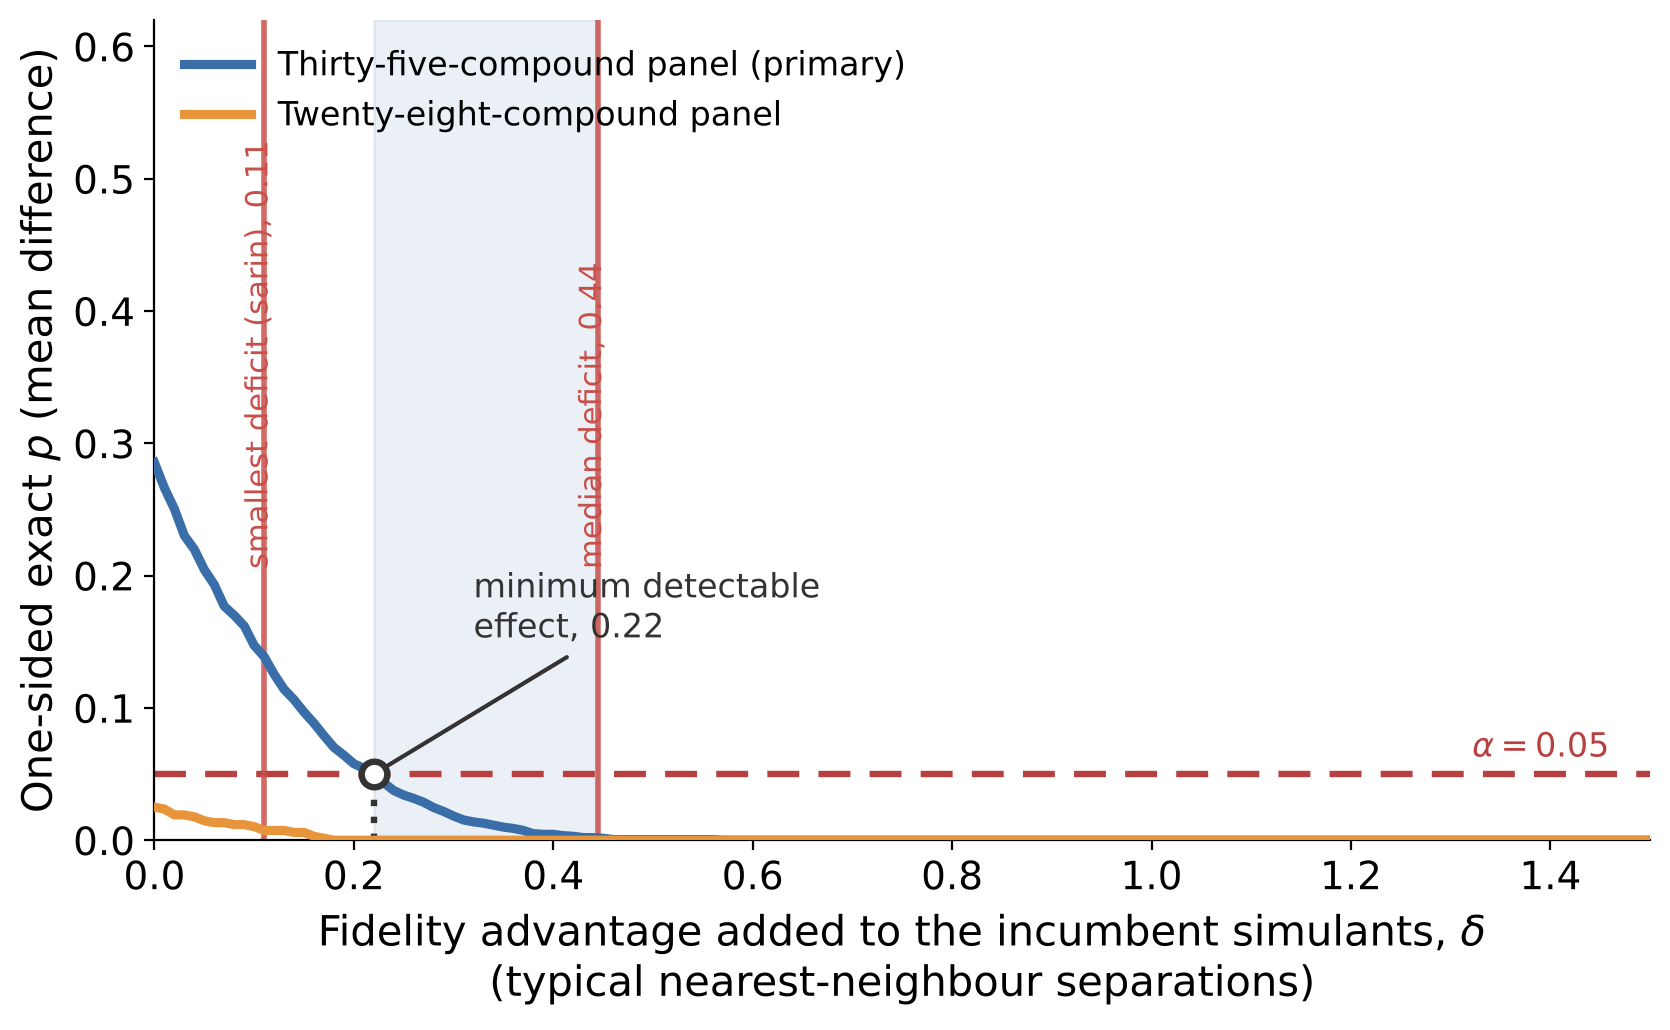
\includegraphics[width=\textwidth]{Fig_mde.png}
\caption{What the permutation test could have detected. One-sided exact $p$ for
the mean-difference statistic as the incumbent simulants are moved $\delta$
typical nearest-neighbour separations closer to the eleven agents, with the rest
of each panel unchanged and the null taken from the unmodified distances. On the
primary panel the test crosses $\alpha = 0.05$ at $\delta = 0.23$. The shaded
band spans that value and the median deficit the incumbent compounds actually
carry, 0.493; the deficit falls below the detectable value only at sarin.}
\label{fig:mde}
\end{figure}

\begin{figure}[t]
\centering
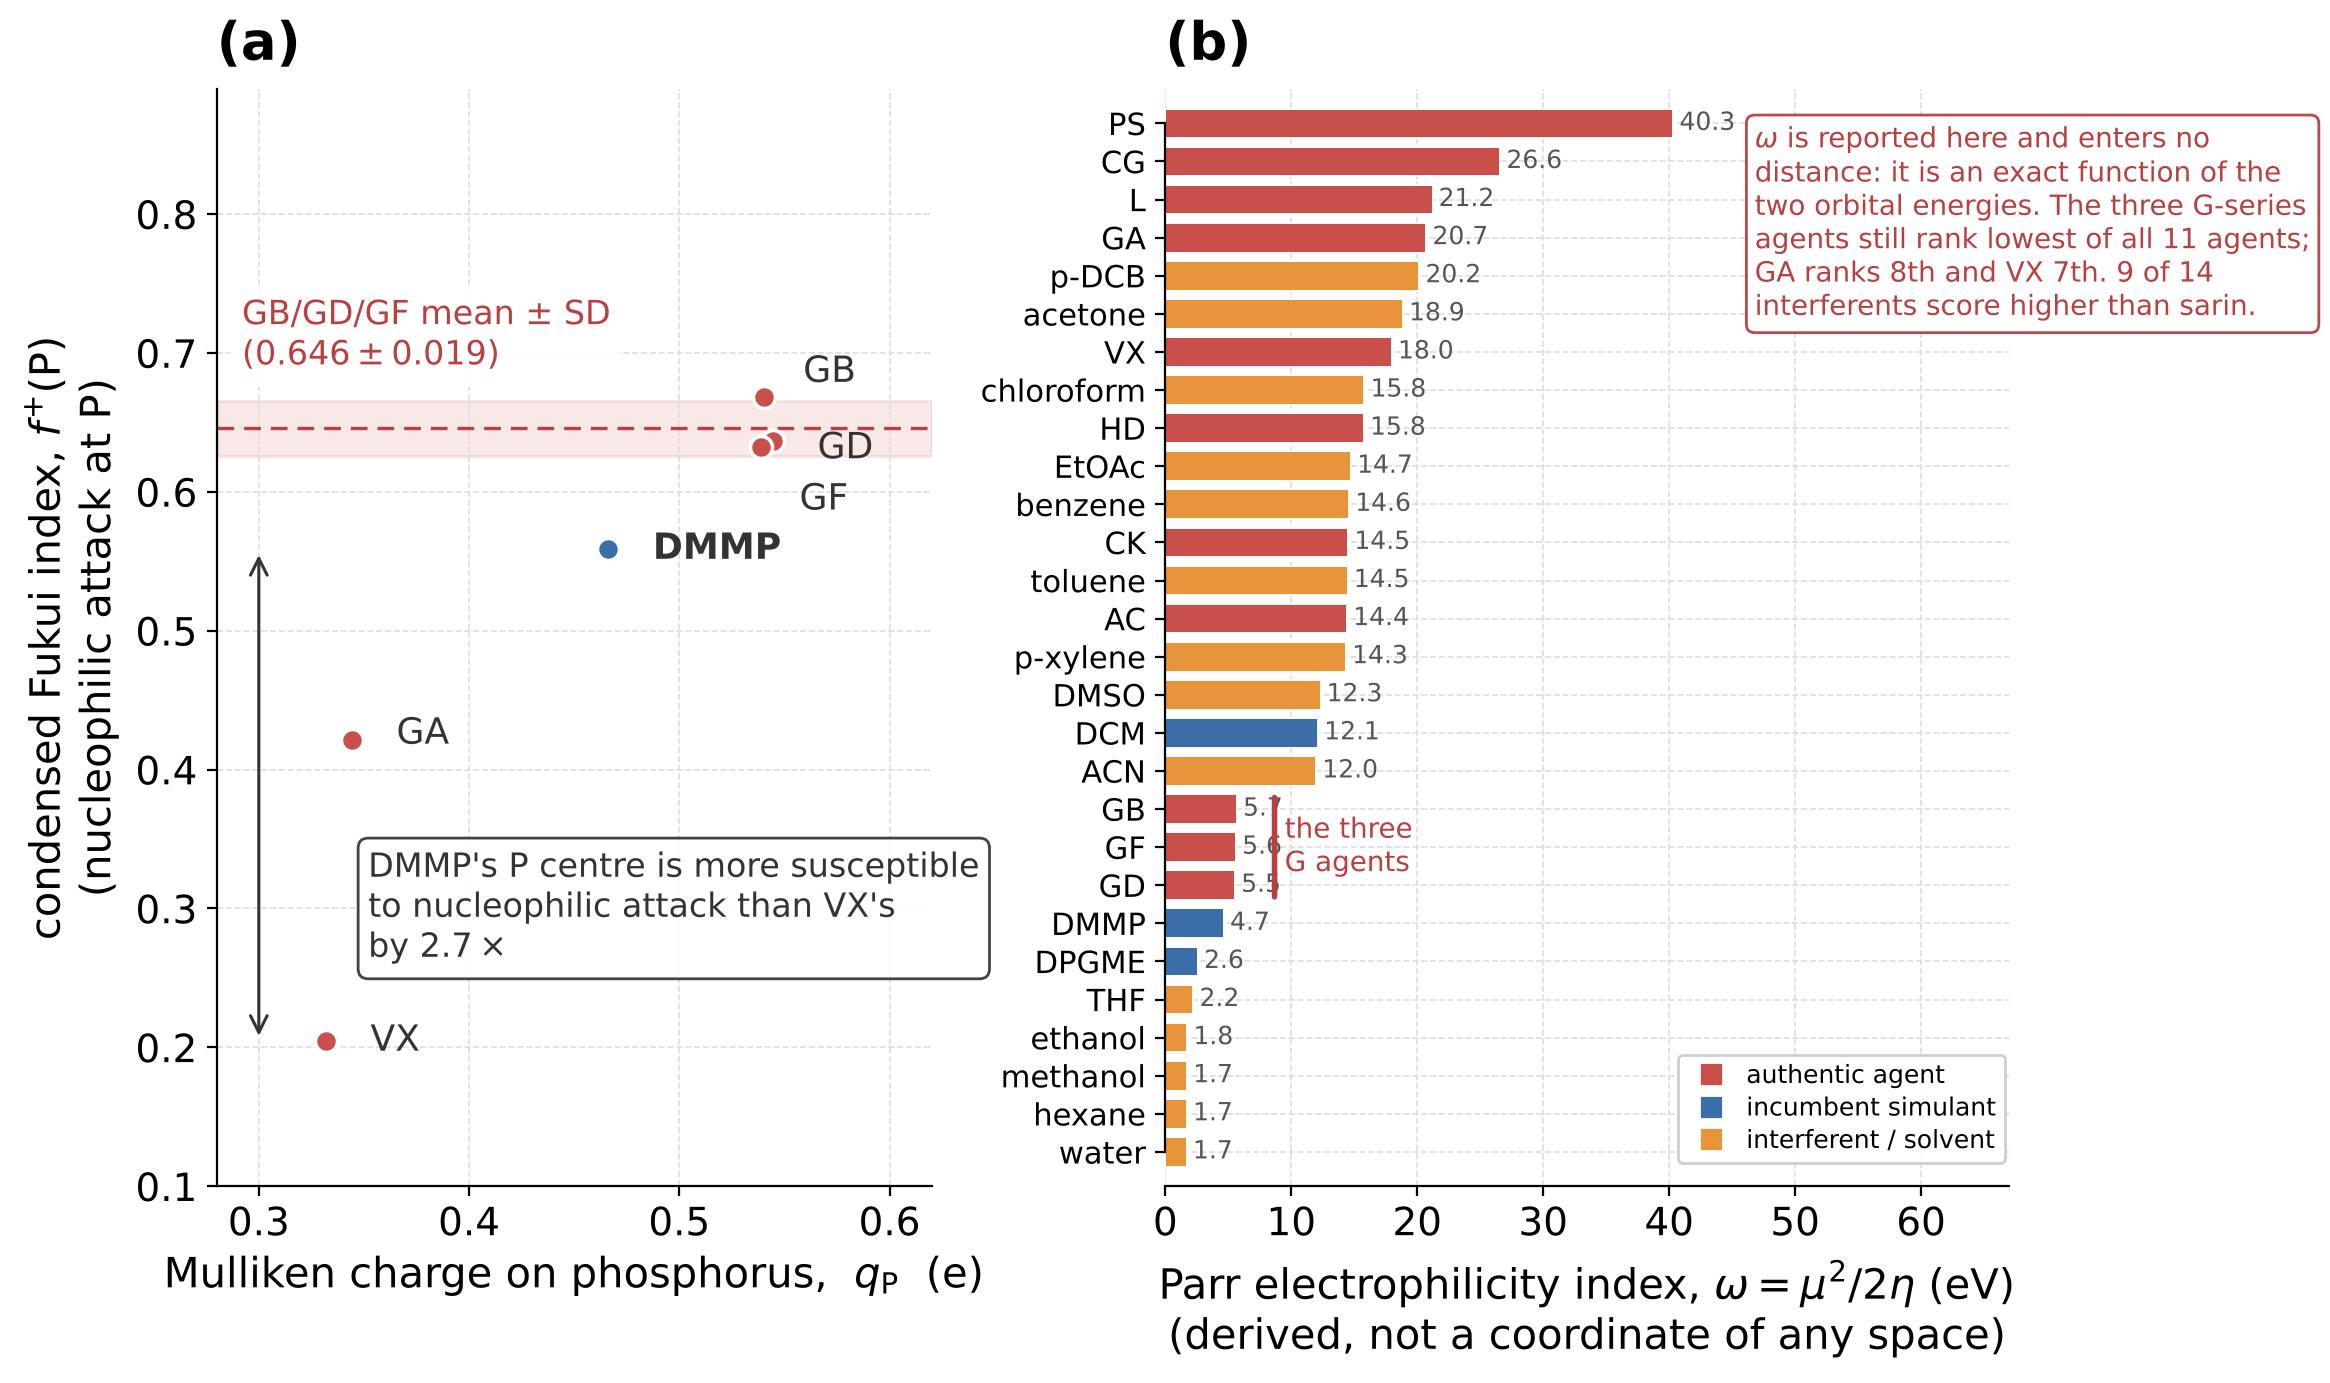
\includegraphics[width=\textwidth]{Fig_plocal.png}
\caption{Two quantities that sit outside every distance used in this work.
(a) Local electrophilicity against Mulliken charge at phosphorus for the six
phosphorus-bearing compounds (Section~\ref{res:plocal}). (b) The Parr
electrophilicity index, an exact function of the orbital energies that enter the
electronic space, which itself enters no distance anywhere in this work
(Section~\ref{M-meth:spaces}) and on which the three nerve agents rank lowest of
the eleven agents. The principal components of the two spaces are not
reproduced here.}
\label{fig:plocal}
\end{figure}

\section{Local reactivity at phosphorus}
\label{res:plocal}

Table~\ref{tab:plocal} gives the phosphorus-centred quantities. The relevant
reactivity is the attack of the serine hydroxyl of acetylcholinesterase on
phosphorus, so the quantity of interest is the susceptibility of that centre to
a nucleophile, which is what $f^{+}(\mathrm{P})$ measures.

$f^{+}(\mathrm{P})$ orders GB $>$ GD $>$ GF $>$ DMMP $>$ GA $>$ VX. DMMP reaches
84\% of sarin's value but lies 4.47 standard deviations below the tight GB/GD/GF
cluster ($0.6456 \pm 0.0195$), so it is the closest available compound rather
than a member of the group. Against VX, DMMP's $f^{+}(\mathrm{P})$ is 2.73 times
larger.

That last ratio depends on which quantity is taken to represent local
reactivity, and we report both because they disagree. The composite local
electrophilicity of Domingo et al.~\cite{domingo2016},
$\omega_k = \omega f^{+}_k$, weights the condensed Fukui index by the global
index, and under it DMMP reaches 0.69 of sarin and 0.71 of VX rather than 2.73
times VX: the direction of the DMMP--VX comparison reverses. The reversal is
carried entirely by the global factor, which for VX is 17.99~eV because the
sulfur lone pair raises the HOMO, and for tabun 20.73~eV because of the nitrile.
Those are the same values that the next paragraph shows to be unusable as a
reactivity ordering for this compound class, so we do not treat $\omega_k$ as
the arbiter; but a reader applying the standard composite to Table~\ref{tab:plocal}
would reach the opposite conclusion about VX, and that is worth stating plainly.
Against the GB/GD/GF cluster the two conventions agree and $\omega_k$ is the
harsher of the two, placing DMMP 6.87 standard deviations below the cluster
against 4.47 for $f^{+}(\mathrm{P})$ alone.

The measured array response bears on this and narrows it.
Section~\ref{res:arraydetail} compares DMMP's 29-dye response pattern with those of
the authentic agents. DMMP is closer to sarin than to VX by 1.35 in cosine in
the ultraviolet channel and by 0.84 in reflectance, both intervals excluding
zero, so on the VX comparison the measurement sides with $f^{+}(\mathrm{P})$
against $\omega_k$. It does not support the wider reading that DMMP stands in
for the G series as a class: GD and GF are both further from DMMP than VX is.

\begin{table}[!htb]
\centering
\caption{GFN2-xTB local reactivity at phosphorus for the six phosphorus-bearing
compounds. $f^{+}(\mathrm{P})$ is the condensed Fukui index for nucleophilic
attack at phosphorus, in the frontier-electron formulation of Parr and
Yang\cite{parryang1984} with the atomic condensation of Yang and
Mortier.\cite{yangmortier1986} $\omega$ is the global electrophilicity index in the
definition of Parr et al.~\cite{parr1999} with $\eta$ equal to half the
HOMO--LUMO gap, and $\omega_k = \omega f^{+}(\mathrm{P})$ is the composite local
electrophilicity of Domingo et al.~\cite{domingo2016}. The two reactivity
conventions disagree about VX and the text says why.}
\label{tab:plocal}
\small
% 자동 생성 — make_si_tables.py. 손으로 고치지 말 것.
\begin{tabular}{lcccccc}
\hline
Compound & $q_{\mathrm{P}}$ (e) & $q_{\mathrm{P=O}}$ (e) & $W_{\mathrm{P=O}}$ &
$f^{+}(\mathrm{P})$ & $\omega$ (eV) & $\omega_k$ (eV) \\
\hline
GB & 0.54044 & -0.42847 & 1.9527 & 0.66793 & 5.69 & 3.80 \\
GD & 0.54460 & -0.43006 & 1.9507 & 0.63692 & 5.54 & 3.53 \\
GF & 0.53868 & -0.42662 & 1.9546 & 0.63203 & 5.62 & 3.55 \\
\textbf{DMMP} & 0.46630 & -0.44588 & 1.9246 & 0.55852 & 4.66 & 2.60 \\
GA & 0.34433 & -0.38982 & 2.0146 & 0.42143 & 20.73 & 8.74 \\
VX & 0.33196 & -0.40303 & 1.9863 & 0.20431 & 17.99 & 3.68 \\
\hline
\multicolumn{7}{l}{\footnotesize GB/GD/GF mean $f^{+}(\mathrm{P})$ = 0.6456
$\pm$ 0.0195, DMMP 4.47 SD below; mean $\omega_k$ = 3.63 $\pm$ 0.15,}\\
\multicolumn{7}{l}{\footnotesize DMMP 6.87 SD below. $\omega$ and $\omega_k$ are
reported here and used in no distance (Section~\ref{M-meth:spaces}).}\\
\multicolumn{7}{l}{\footnotesize DMMP/VX = 2.73 by $f^{+}(\mathrm{P})$ but 0.71 by
$\omega_k$. Values are GFN2-derived and relative within one protocol.}\\
\end{tabular}

\end{table}

The Wiberg P=O bond order,\cite{wiberg1968,mayer1983} which spans
1.9246--2.0146 across all six compounds, does
not separate the G series from DMMP; it carries no useful discrimination here.
The global electrophilicity index does not order this panel in a way that
tracks agent reactivity, and it does not order it reproducibly either. Under
GFN2 the three lowest values among the eleven authentic agents are GD (5.54),
GF (5.62) and GB (5.69), and nine of the fourteen interferents score higher
than sarin. The reason $\omega$ behaves this way is that it responds to the
lowest $\pi^{*}$ orbital wherever it sits, the nitrile in tabun or the sulfur
lone pair raising the HOMO in VX, and it has no particular connection to
phosphorus.

That much is a statement about $\omega$. Whether it is also a statement about
GFN2 is a separate question, and it has to be asked, because the GFN2 values
themselves are not credible as electrophilicity indices: they run from 1.71 to
40.34~eV across this panel, where a density-functional calculation on organic
molecules of this kind returns single-digit values. We recomputed the whole
twenty-eight-compound panel at B3LYP/def2-SVPD (Section~\ref{meth:dft}). The
range becomes 1.43 to 7.92~eV, chloropicrin falling from 40.34 to 7.92 and
phosgene from 26.60 to 5.07, and the inflation factor is not constant: it runs
from 0.7 for water to 11.7 for VX.

Two things follow, and they point in opposite directions for us. The qualitative
reading survives. Under the density-functional values the simulant still does
not sit above the agents it stands in for, DMMP at 1.90 against sarin at 2.08,
and seven of the fourteen interferents still score above sarin, so $\omega$
still fails to separate this panel in the way a reactivity axis would need to.
The specific ordering does not survive. The three lowest agents become VX
(1.54), sulfur mustard (1.73) and cyclosarin (1.90) rather than the G series,
and two agents now fall below DMMP where under GFN2 all eleven stood above it.
The rank correlation between the two sets of $\omega$ values is 0.628, against
0.898 for the underlying LUMO energies, which is what one expects of a quantity
that divides by a gap: the construction amplifies the disagreement rather than
inheriting it.

We therefore keep the conclusion and withdraw the ordering. Global
electrophilicity should not be used as a reactivity axis for this compound
class, and the sentence we would have written before this check, naming which
three agents sit lowest, would have been a statement about the semi-empirical
method rather than about the compounds.

\section{What the array actually measures}
\label{res:arraydetail}

Every argument above rests on descriptor distances, and the premise that one of
those spaces corresponds to what a vapour-phase sensor reports has so far been
assumed rather than shown. We test it against measured response from a
29-dye colorimetric array, reported for three compound sets at four
concentrations in two imaging channels, ultraviolet-excited and reflectance
(Section~\ref{meth:deltaE}). Twelve of the measured compounds are in the panel:
DMMP and the five nerve agents in the first set, and six of the remaining agents
in the second.

The array discriminates, but only after the common-mode response is removed, and
less of that separation is empirical than the raw numbers suggest. Colour
difference is a non-negative quantity, so every analyte shares a common
``something responded'' component and cosine similarity between raw profiles is
compressed towards unity. Between-compound similarity of 0.77 to 0.80 is not
separable from the within-compound value of 0.79 to 0.83 across concentrations
($p = 0.06$ to $0.94$). Subtracting the compound-axis mean at each concentration
separates them, to $+0.3451$ to $+0.5416$ within compounds against $-0.1026$ to
$-0.3302$ between them, in all six combinations of compound set and channel.

The sign-flip enumeration we pre-specified for this contrast returns the
smallest value each compound count allows in every cell, from 0.0078 to 0.0625,
and Section~\ref{meth:deltaE} withdraws it. The test reported below permutes
compound labels within each concentration. The statistic is unchanged, the mean
over compounds of the within-concentration agreement minus the
between-compound agreement, and only the null changes.

\begin{table}[!htb]
\centering
\caption{Premise test under the label-permutation null. The statistic is the
mean over compounds of (agreement with itself across concentrations) minus
(agreement with the other compounds' consensus patterns). The null permutes
compound labels within each concentration. Fixing the first concentration's
labels leaves $(n!)^{C-1}$ distinct relabellings, which is enumerable for the
four-compound set and sampled for the others.}
\label{tab:premisenull}
% 자동 생성 — make_si_tables.py. 손으로 고치지 말 것.
\begin{tabular}{llrrrrl}
\hline
Set & Channel & Observed & Null mean & Null s.d. & $p$ & Null built from \\
\hline
First & ultraviolet & $+0.7288$ & $+0.1571$ & 0.1013 & 0.0001 & 10,000 sampled \\
First & reflectance & $+0.6931$ & $+0.1497$ & 0.0845 & 0.0001 & 10,000 sampled \\
Second & ultraviolet & $+0.5578$ & $+0.1024$ & 0.0903 & 0.0001 & 10,000 sampled \\
Second & reflectance & $+0.6187$ & $+0.1109$ & 0.0654 & 0.0001 & 10,000 sampled \\
Third & ultraviolet & $+0.5669$ & $+0.1898$ & 0.1442 & 0.0046 & 13,824 enumerated \\
Third & reflectance & $+0.6753$ & $+0.3138$ & 0.1025 & 0.0033 & 13,824 enumerated \\
\hline
\multicolumn{7}{l}{\footnotesize Adjusted values are Benjamini--Hochberg over the six cells; the smallest is }\\
\multicolumn{7}{l}{\footnotesize 0.0001 and all six clear $q=0.05$.}\\
\end{tabular}

\end{table}

Table~\ref{tab:premisenull} gives the result. All six cells clear
$q = 0.05$, the smallest adjusted value being 0.0001, and the null mean is
positive in every cell rather than zero. That positive null mean is the
quantity the withdrawn floor argument was reaching for: it says how much of
the observed difference centring produces on its own, between $+0.1024$ and
$+0.3138$ against observed values of $+0.5578$ to $+0.7288$. The reflectance
channel of the third run, which the floor comparison discarded for sitting
$0.0032$ above $-1/3$, has the largest null mean of the six and still clears
the threshold.

Two limits stay. The contrast holds per compound on average and not pairwise:
in 13 of the 34 compound-and-cell instances some other compound's consensus is
closer than the compound's own agreement across concentrations. And the
sampled cells give a resolution of $10^{-4}$ in $p$, so the four sampled
values are upper bounds on how small those values are rather than estimates of
them. All results below use the centred patterns, with those caveats attached.

% 2026-11-03 (T1-13). 종전에는 바닥이 네 셀에서만 계산되어 있었다. d3 두
% 셀이 Mantel 관문 뒤에 있어 빠졌고, 빠진 셀 하나가 여유 최소값이다.
% 수치는 outputs/rollback_c.json 의 deltaE.centring_floor 실측.

The measurement bears on Supplementary Section~\ref{res:plocal}, and it narrows the claim
rather than confirming it. What replicates across both channels is specific to
sarin. DMMP's pattern is closer to GB than to VX by 1.347 in cosine in the
ultraviolet channel (95\% CI 1.062 to 1.436, bootstrapped over concentrations)
and by 0.841 in reflectance (0.462 to 0.903), and closer to GB than to the mean
of GD, GF and VX by 1.284 and 0.984 in the two channels, every interval
excluding zero. The class-level statement is weaker. Taking the mean of the
three matched G agents against VX gives 0.513 (0.131 to 0.722) in the
ultraviolet channel but 0.137 (-0.144 to 0.290) in reflectance, and the least
similar agent to DMMP is GF rather than VX in both channels (-0.721 and -0.496
against -0.702 and -0.273 for VX).

The full ranking contains one result that the descriptor analysis does not
anticipate, and we give the whole ranking rather than the comparison we set out
to make. In the ultraviolet channel the agent nearest to DMMP is not sarin but
tabun, at $+0.764$ against sarin's $+0.645$, with soman, VX and cyclosarin
following at $-0.492$, $-0.702$ and $-0.721$. In reflectance sarin leads at
$+0.569$ and tabun falls to $-0.112$. Tabun sits on the descriptor criterion of
Section~\ref{M-res:panels} rather than inside it: its normalised distance is
2.0038 against a threshold of 2, where sarin sits at 1.187, and
Section~\ref{meth:orderinvariance} shows that implementation choices carrying no
chemical content move it to either side of that threshold. The descriptor table
therefore does not count tabun among the matches, while the measured ultraviolet
channel places it first of the five agents. The two do not disagree about a
settled count. They disagree about the order, and they disagree most about the
one agent the descriptor criterion cannot resolve. The measured channel in which the
ordering is clearest puts tabun first, the descriptor table puts it last of the
four, and the agreement between the two channels on tabun is the worst of any
agent in the set.
We report this as a disagreement between the descriptor table and the measurement
and not as a correction to either, because two channels on one plate set cannot
settle which is right.

The descriptor analysis assigns GB, GD and GF to DMMP and leaves GA on the
threshold. The array places sarin first in one channel and tabun first in the
other, and does not place GD or GF closer to DMMP than VX in either. A sensor chemistry calibrated on DMMP is
therefore being shown something that behaves like one G agent at a time, not like
the G series, and the descriptor match for the other two does not survive contact
with the measured response.

It does not answer the larger question in either direction. Pattern
dissimilarity, taken as $1 - \cos$ and correlated against descriptor distance,
gives the same inconsistent picture as the permutation tests of
Section~\ref{M-res:panels}. Tested by Mantel permutation over compounds
(Section~\ref{meth:deltaE}), three of the twelve panel-channel-space cells reach a
nominal $p<0.05$, and they do not agree on a space: the merged space in the
second compound set's ultraviolet channel ($\rho = +0.500$, Mantel $p = 0.019$),
the structural space in that same set and channel ($\rho = +0.511$, Mantel
$p = 0.017$),
and the electronic space in the same set's reflectance channel ($\rho = +0.571$,
Mantel $p = 0.044$). The first compound set gives nothing in any space or
channel ($|\rho| \le 0.225$, Mantel $p \ge 0.22$).

Which set the three nominal cells come from decides what they can mean, and we
state it because the composition of the two sets is not symmetric. The first set
is DMMP with five G agents and VX, and it is the only one of the two that
contains a simulant at all; the second is seven authentic agents and no
simulant. A cell in the second set therefore asks whether the pattern distance
between two agents tracks their descriptor distance, which is a different
question from whether a simulant stands in for an agent. All three nominal cells
are in the second set. The six cells that bear directly on the premise this
paper rests on are the six in the first set, and all six are null. We have not
shown that the descriptor spaces fail to predict simulant-to-agent response; we
have shown that the only measurement able to address it does not address it, on
six compounds, at a resolution that would have needed a near-deterministic
association to register. The twelve cells are one
family, and we correct them as we correct the permutation tests of
Section~\ref{M-res:panels}: under Benjamini-Hochberg the smallest adjusted value is
0.117 and no cell reaches $q<0.05$. We state the nominal values as well because
cells pointing at different descriptor spaces is itself the pattern worth
seeing, but no cell is a result. An earlier version of this analysis ran the
Mantel test in the structural and electronic spaces only and corrected over the
resulting eight cells. The merged space is the one the rest of this paper leads
with, and the cell it contributes is the strongest of the twelve, so omitting it
narrowed the family after the fact and in the direction that weakened the
association. Restoring it moves the smallest adjusted value from 0.133 to
0.117.

Not every declared channel is a separate measurement, and in one plate set six of
them are not. In the second set's ultraviolet channel, dyes 22 to 27 return
values identical to the last decimal place in every row. The images behind them
are distinct files, so this is not a naming collision; the six dyes do not
fluoresce under ultraviolet illumination and the region of interest read plate
background instead. One background channel was therefore entering the unit-
normalised pattern six times. Two further columns in the same channel, and five
in the third set's, are identically zero. We collapse columns that are equal in
every row to a single occurrence, a rule declared once and applied to all six
plate-channel combinations, which leaves 23 effective channels in the second
set's ultraviolet data and 25 in the third set's, against 29 elsewhere. The
collapse weakens the two cells it touches, from $\rho = +0.568$ and $+0.539$ to
$+0.518$ and $+0.496$, and moves the smallest adjusted value over the twelve
cells from 0.067 to 0.124. We report the collapsed values throughout, because a
paper arguing that analyst choices inflate results cannot keep a sixfold
duplicate that happens to fall in its two strongest cells. Which columns were
collapsed is recorded in the deposited output.

Treating the fifteen pairs as independent observations, which the first version
of this analysis did, moves these values by up to 0.038 and in both directions:
it would have reported the structural cell at $p = 0.052$ rather than 0.017 and
the merged cell at 0.058 rather than 0.019. The error is not large here
because the sets are small, but it is the error that would grow with panel size,
and in the electronic cell it runs the other way, to 0.026 from 0.044.

Pooling the two compound sets by Fisher transformation, which is legitimate
because they are different compounds on different plates, the structural space
gives $\rho = +0.306$ (95\% CI $-0.450$ to $+0.806$) in the ultraviolet channel
and $+0.141$ ($-0.577$ to $+0.736$) in reflectance, while the electronic space
gives $-0.107$ ($-0.720$ to $+0.600$) and $+0.327$ ($-0.431$ to $+0.814$). The
weight here is $n-3$ with $n$ the six compounds, not the fifteen pairs they
generate; the earlier version of this section used the pairs, which is the error
it criticises two paragraphs above and which narrowed every interval by roughly
a factor of two. Every interval contains zero. The electronic space is the
better predictor in one of the four cells.

Six compounds per set bound how much that null can carry, and bounding it
correctly took us two attempts. A Fisher $z$ calculation on the fifteen pairs
returns $|\rho| \ge 0.669$ at 80\% power; the same calculation with the six
compounds as the unit, which is the unit the Mantel test uses, returns $0.924$.
Neither is the test we ran. The cell test enumerates all $6! = 720$ relabellings
of the compounds, and that permutation null is narrower than one built from
independent pairs, because it preserves the dependence among the fifteen pairs
rather than ignoring it. A narrow null compensates for a small sample, so the
approximation at the correct unit understates the power of the procedure. We
therefore simulated the procedure itself (Section~\ref{meth:deltaE}): at
$\alpha = 0.05$, 80\% power is reached at $|\rho| = 0.67$, with the type~I rate
of the simulated test at 0.049 against a nominal 0.05. The smallest attainable
$p$ is $1/720$, so the resolution is coarse but not as coarse as the
compound-unit approximation suggests. These data exclude a strong association
between either descriptor space and the measured response and nothing weaker. They do not show that the
electronic space governs sensor response, do not place it above the structural
space, and do not show it to be irrelevant. The claims in the rest of this paper
are written to that limit.

\section{The measured safety axis, and the holes in it}

Nineteen of the twenty-eight compounds have an AEGL-3 at 10~min
(Fig.~\ref{M-fig:tox}a). The ordering runs VX (0.0295~mg~m$^{-3}$), soman (0.365),
sarin (0.367), cyclosarin (0.391), tabun (0.729), sulfur mustard (3.84),
lewisite~1 (3.9), chloropicrin (13.4), phosgene (14.6), hydrogen cyanide (29.8),
acetonitrile (403), chloroform (19\,530), benzene (30\,990), p-xylene (31\,264),
toluene (37\,685), acetone (38\,007), dichloromethane (41\,685), n-hexane
(42\,296) and methanol (52\,420). The axis spans six orders of magnitude, and
the incumbent simulant dichloromethane sits at the safe end of it,
$1.4\times10^{6}$ times less acutely toxic than VX and 1400 times less toxic
than hydrogen cyanide. On this axis the incumbent simulant is not the weak link.

It is, however, not the safest thing on the panel. Methanol and n-hexane both
carry higher AEGL-3 values than dichloromethane, and neither is used as a
simulant for anything. The point is not that either should be: it is that the
safety axis cannot be what selected the incumbent, because two ordinary
laboratory solvents on the same panel score better on it. Against the 207 AEGL
compounds that carry both axes (Section~\ref{res:h1}) dichloromethane sits at
the 96th percentile of measured acute inhalation safety, with seven compounds
above it. Taking the incumbent as the bar a replacement must meet therefore sets
a demanding bar, and the consequences are worked through in
Section~\ref{res:h1}.

Nine compounds have no value. Eight are absent from the AEGL list altogether:
DMMP, tetrahydrofuran, ethyl acetate, water, DPGME, ethanol, DMSO and
p-dichlorobenzene. The ninth, cyanogen chloride, is the one military agent
among them, and its absence is a recorded decision rather than an oversight: it
appears in the compiled table's holding list, where the agency states that
values are not being developed. Checked by CAS against the source document, it
is the only one of the nine on that list. DMMP's position is worth stating
precisely, because it is the compound
that carries all three valid matches found above. EPA's provisional
peer-reviewed assessment declined to derive an inhalation reference
concentration, recording that the data are insufficient, and derived no
inhalation unit risk; no acute inhalation LC$_{50}$ is cited; IRIS and HEAST
contain no RfD, RfC or cancer value. What exists is an oral provisional RfD of
0.06~mg~kg$^{-1}$~day$^{-1}$ carrying an uncertainty factor of 3000, and an oral
cancer slope factor of $1.7\times10^{-3}$ (mg~kg$^{-1}$~day$^{-1}$)$^{-1}$ based
on mononuclear cell leukaemia in male rats, with the evidence characterised as
suggestive \cite{epapprtv2006}. The inhalation safety of the field's principal
nerve-agent simulant has not been established; it has not been assessed. The two
incumbent simulants therefore sit at opposite ends of the evidence, not of the
hazard: for dichloromethane there is a regulator-derived value and it is
favourable, and for DMMP there is a regulator's recorded decision not to derive
one.

Cyclosarin carries its own entry in the compiled table under CAS 329-99-7, with
a ten-minute AEGL-3 of 0.053~ppm bracketed by the agency as 0.38~mg~m$^{-3}$;
our conversion from the published parts-per-million value gives
0.39~mg~m$^{-3}$, placing it between sarin and tabun. The entry is titled
\textit{GF Agent} rather than \textit{Agent GF}, which is why matching on
compound names rather than on registry numbers can miss it;
Section~\ref{meth:aegl} describes the CAS-keyed procedure used here.

\section{A QSAR cannot fill the gaps}
\label{res:qsar}

On the training distribution the model works. The random forest
(Fig.~\ref{M-fig:tox}b) reached $R^{2}=0.458 \pm 0.014$ and RMSE $0.935$ in
$\log_{10}$ units (95\% CI 0.830--1.020) against a training-mean baseline of
1.271 (1.175--1.365) and a logP-plus-molecular-weight linear baseline of 1.225.
The intervals for the model and the mean baseline do not overlap, and the
out-of-fold error over the whole training set is unbiased, averaging $+0.001$ log
units. Nothing in the cross-validated statistics would warn a user off.

On the twenty agents held out of training it failed, in one direction and without
exception. Every one was predicted safer than measured, by between 0.40 and 3.42
log units, a factor of 2.5 to 2600. Sarin was placed at 29~mg~m$^{-3}$ against a
measured 0.367 and VX at 2.4 against 0.0295, errors of 79-fold and 80-fold.
Fourteen of the twenty lie inside the applicability domain, so for those the
domain check raises no objection, and the worst of those fourteen is still wrong
by 2.68 log units, a factor of 482. DMMP's domain distance, 3.28, sits among the
agents' own, which is to say inside the region where the model is wrong by one to
two orders of magnitude, so its prediction is not used.

\begin{sloppypar}
The explanation is not that the mechanism is missing from the training set. We
checked, because that was our first hypothesis and it is wrong. Thirteen of the
230 training compounds carry an acetylcholinesterase-inhibiting pharmacophore,
identified by substructure rather than by name: ten organophosphorus esters
(phorate, phosphamidon, monocrotophos, dicrotophos, fenamiphos, parathion,
methyl parathion, methamidophos, dichlorvos, malathion) and three carbamate
esters (aldicarb, oxamyl, methomyl). The mechanism by which the nerve agents
kill, phosphylation of the serine hydroxyl of acetylcholinesterase and the
cholinergic crisis that follows \cite{bajgar2004,thiermann2013,worek2020},
is therefore represented, and one of
the thirteen, phorate at 0.22~mg~m$^{-3}$, is more acutely toxic than sarin. The
model sees the mechanism and still cannot place the agents.
\end{sloppypar}

What it cannot do is reach either extreme. Over the whole training set the
out-of-fold error is centred on zero, but in the most toxic decile
(the 23 compounds at or below 3.21~mg~m$^{-3}$) it averages $+1.41$ log units
and is positive for every single compound, while in the least toxic decile (the
23 at or above 8094~mg~m$^{-3}$) it averages $-1.13$ log units and is negative
for all but one. The same symmetry appears inside the anticholinesterase subset
taken on its own: phorate, the most toxic of the thirteen, is predicted 177 times
too safe, while malathion, the least toxic, is predicted 269 times too toxic.
This is regression toward the mean at both tails, which is what a
variance-minimising ensemble does with sparsely populated extremes, and the
agents are all in one of them.

That diagnosis matters for the applicability domain rather than for the model.
A descriptor-distance domain asks whether a compound is unusual in the space of
inputs. The failure here is defined in the space of the response, and the two do
not coincide: fourteen of twenty agents are ordinary-looking inputs with
extreme outputs. An input-space criterion cannot detect an output-space bias, so
it certifies exactly the predictions that are worst. This is the same failure, in
the safety axis, that Section~\ref{M-res:panels} documents in the fidelity axis.
A distance in one space is being used to vouch for a property that lives in
another.

\begin{figure}[t]
\centering
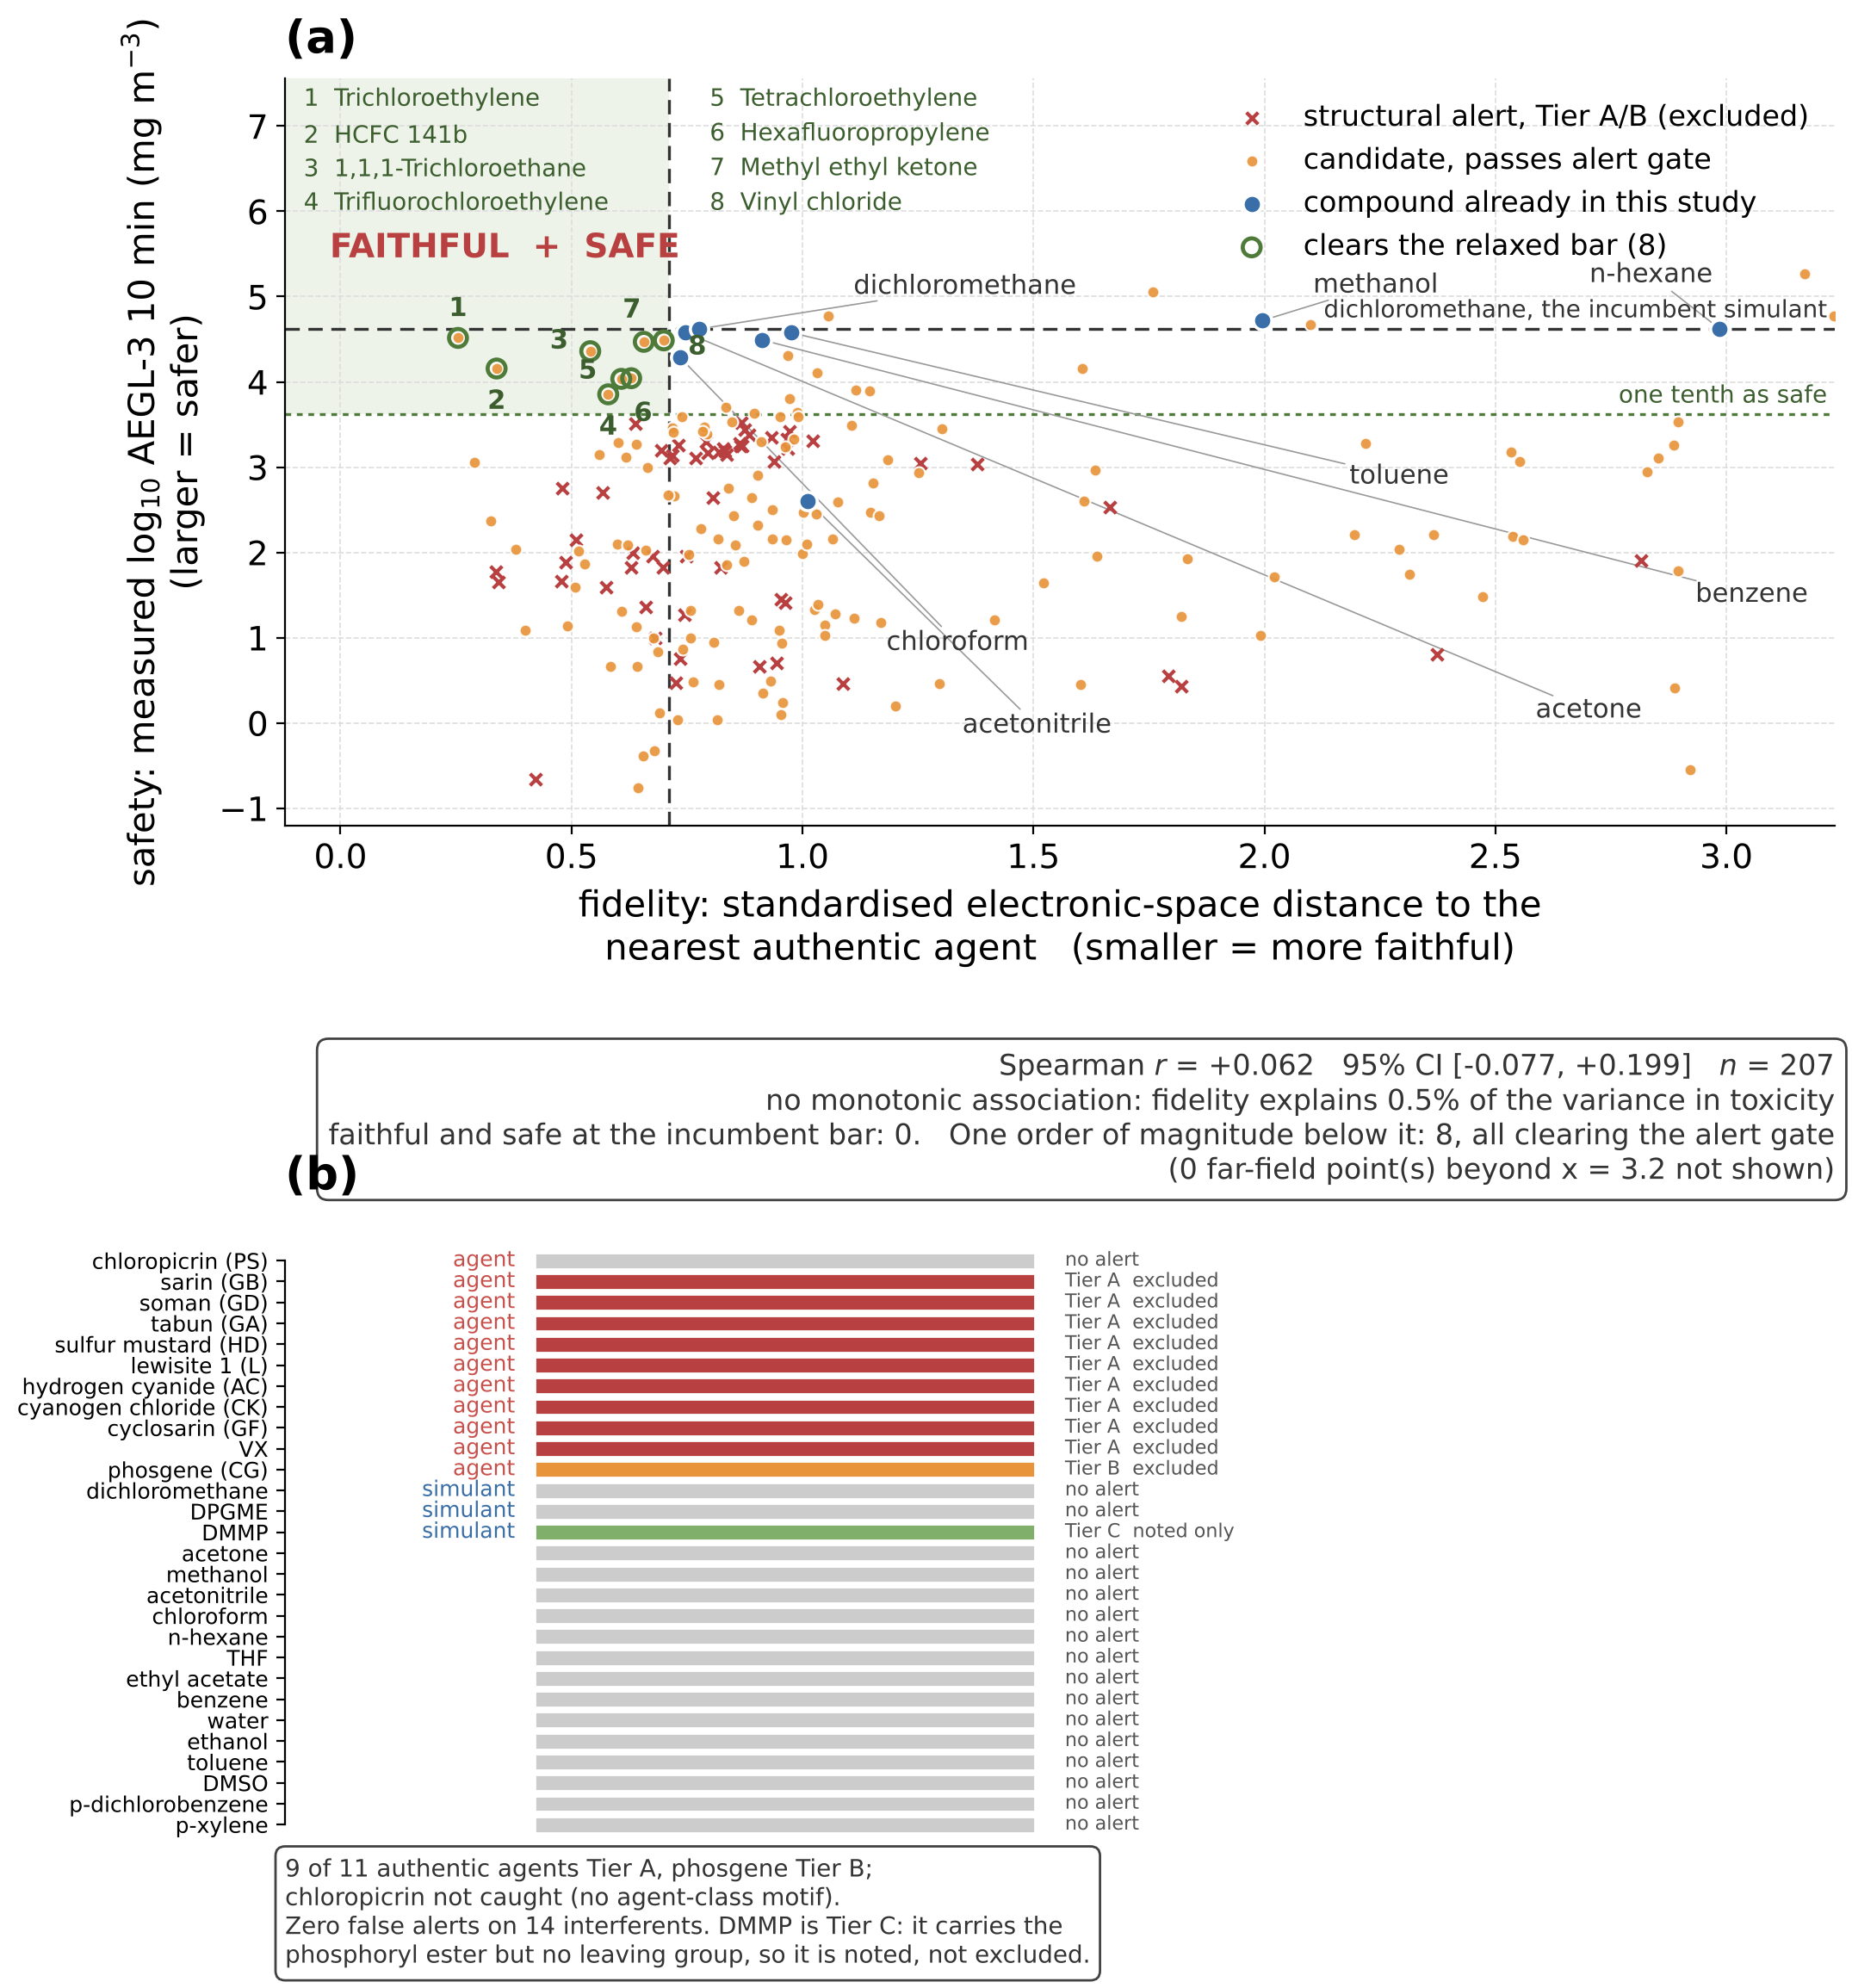
\includegraphics[width=\textwidth]{Fig_h1.png}
\caption{Fidelity and safety are not monotonically associated. (a) Electronic-space distance to
the nearest authentic agent against measured AEGL-3 for the 207 candidates
carrying both axes; crosses are compounds excluded by the structural filter. The
upper dashed line is the measured AEGL-3 of dichloromethane, the incumbent
simulant; the dotted line is one order of magnitude below it, and the eight
circled compounds are those that clear the lower bar while also falling in the
most faithful quartile, numbered by fidelity and named at the top left. The
shaded quadrant, faithful and safe at the incumbent's own bar, is empty.
(b) The filter applied to the twenty-eight-compound set: nine of eleven
authentic agents are Tier~A and phosgene Tier~B, there are no false alerts among
the interferents, and DMMP is Tier~C.}
\label{fig:h1}
\end{figure}

\section{Fidelity and safety are not monotonically associated}
\label{res:h1}

Across the 207 candidates carrying both measured axes (Fig.~\ref{fig:h1}a),
fidelity and safety are uncorrelated: Spearman $r=+0.062$ (95\% CI $-0.077$ to
$+0.199$), Pearson $r=+0.072$ (95\% CI $-0.092$ to $+0.225$, $p=0.30$), with
fidelity accounting for 0.5\% of the variance in toxicity
(Table~\ref{tab:h1}). The Spearman interval rules out any monotone association
stronger than $|r|=0.199$ and the Pearson interval any linear association
stronger than $|r|=0.225$, so this is a bounded negative result rather than an
underpowered one. Resembling an agent electronically does not require being as
dangerous as one.

\begin{table}[!htb]
\centering
\caption{Decoupling test. Fidelity is the standardised electronic-space distance to
the nearest authentic agent; safety is the measured EPA AEGL-3 (10~min).}
\label{tab:h1}
\small
\begin{tabular}{lc}
\hline
Quantity & Value \\
\hline
Candidates with both axes measured & 207 \\
Spearman $r$ & $+0.062$ (95\% CI $-0.077$ to $+0.199$) \\
Pearson $r$ & $+0.072$ (95\% CI $-0.092$ to $+0.225$), $p = 0.30$ \\
Variance of toxicity explained by fidelity & 0.5\% \\
\hline
Safety bar: dichloromethane, 41,685~mg~m$^{-3}$ & $\log_{10} = 4.62$ \\
Faithful and safe at that bar & 0 \\
Faithful and safe one order of magnitude below it & 8 \\
\quad clearing the structural-alert gate & 8 \\
\quad more faithful than dichloromethane itself & 8 \\
Most faithful of them & Trichloroethylene (0.25 vs 0.78) \\
\hline
\end{tabular}
\end{table}

Setting the safety bar at the incumbent simulant's own measured value empties the
faithful-and-safe quadrant outright: of the 207, not one compound combines
top-quartile fidelity with an AEGL-3 at or above dichloromethane's
41\,685~mg~m$^{-3}$, and dichloromethane does not either, its own fidelity of
0.78 falling outside the 0.71 quartile boundary. That is a statement
about how safe dichloromethane is, not about how scarce candidates are. Eight
compounds in the whole pool reach or exceed it on the safety axis, the incumbent
among them, and not one of the eight is faithful.

Lowering the bar by one order of magnitude, to 4168~mg~m$^{-3}$, changes the
answer. Eight compounds then combine top-quartile fidelity with that level of
measured acute inhalation safety, every one of them clears the structural-alert
gate, and every one of them is more faithful than dichloromethane itself. In
order of fidelity they are trichloroethylene (0.25), HCFC~141b (0.34),
1,1,1-trichloroethane (0.54), trifluorochloroethylene (0.58),
tetrachloroethylene (0.61), hexafluoropropylene (0.63), methyl ethyl ketone
(0.66) and vinyl chloride (0.70), every one of them ahead of dichloromethane's
own 0.78. The best of them,
trichloroethylene, is 3.1 times closer to the nearest authentic agent in the
electronic space while being only 1.3 times more acutely toxic by inhalation. At
two orders of magnitude below the incumbent the count rises to fifteen, all of
which clear the gate.

\begin{sloppypar}
These are candidates on the axes measured here, and that qualification is not a
formality. Trichloroethylene and tetrachloroethylene carry serious chronic and
carcinogenic hazard that an acute inhalation criterion does not express, and the
chlorofluorocarbons among them raise questions of atmospheric persistence rather
than of laboratory safety. What the screen establishes is narrower and still
useful: in the electronic space, compounds more faithful than the incumbent
exist at comparable acute inhalation safety, and they were not found by relaxing
the chemistry but by looking in the right descriptor space.
\end{sloppypar}

One limitation bounds this part of the result. The candidate pool is the set of
chemicals for which AEGL values exist, and chemicals receive AEGLs because they
are hazardous. Ordinary safe solvents are largely absent from the pool by
construction, which depresses the count at any bar. The seven compounds that
exceed dichloromethane on the safety axis illustrate the point from the other
side: two are hydrocarbon gases, one a refrigerant, one a monomer, and the three
a laboratory might actually reach for sit far out on the unfaithful side of the
electronic axis, methanol at 2.00 against the 0.71 boundary, well outside the
top quartile that defines a faithful candidate.

\section{The structural filter}

Applied to the 28-compound set (Fig.~\ref{fig:h1}b), the filter assigns Tier~A to nine of the eleven
authentic agents and Tier~B to phosgene, catching ten of eleven; chloropicrin
carries no agent-class motif and is not caught. There are no false alerts among
the fourteen interferents. DMMP is Tier~C: it carries the phosphoryl ester but
not a leaving group, which is precisely why it is used as a simulant and why it
is noted rather than excluded. Dichloromethane and DPGME raise no alert.

The five compounds the primary panel adds have not been put through the filter
anywhere else in this work, and two of them fail it. Diisopropyl
fluorophosphate and diethyl cyanophosphonate carry \texttt{A\_OP\_leaving\_F\_CN},
the same Tier~A alert that catches sarin, soman and cyclosarin; diethyl
chlorophosphate is Tier~C with the phosphoryl ester alone, and methyl
salicylate raises nothing. These are the compounds that displace the incumbents
on the fidelity axis, so the two axes of the criterion point in opposite
directions for them, and nothing here should be read as proposing either as a
replacement. 2-Chloroethyl ethyl sulfide raises no alert at all, which is a
false negative rather than a finding: \texttt{A\_sulfur\_mustard} requires a
2-haloethyl group on both arms of the sulfide, so half-mustards pass a filter
written for the agent. We record it beside chloropicrin as a second known gap
in the filter's coverage. None of the five carries a measured acute inhalation
value in the panel assembled here, so the safety axis is unevaluated for all
of them.


\section{Further discussion of the toxicity axis}
\label{S-disc}

The decoupling result is what makes the rest actionable. Because fidelity and
acute toxicity show no monotonic association across the compounds where both are
measured, the
pursuit of a simulant that is both faithful and safe is not a pursuit along a
trade-off curve, and the screen bears that out. Against the incumbent's own
safety value the quadrant is empty, which says more about dichloromethane than
about the chemistry: it is safer than all but seven of the 207 compounds in the
pool, and not itself faithful enough to fill the quadrant it empties. One order
of magnitude below that bar there are eight candidates, all of
them clearing the structural-alert gate and all of them more faithful than the
incumbent, with trichloroethylene 3.1 times closer to the nearest agent in the
electronic space at 1.3 times the acute inhalation toxicity.

We are not proposing trichloroethylene as a simulant. It carries chronic and
carcinogenic hazard that the axis used here does not express, and a replacement
chosen on two measured axes still has to survive the others. The claim is
narrower and, we think, more useful: the field's incumbent choice is not on the
efficient frontier of the two axes it is usually defended on, and better points
on those axes are already present among compounds with measured toxicity. That
the pool consists of chemicals assessed because they are hazardous depresses
every count reported here, so the seven are a lower bound rather than an
inventory. The constructive reading is that designing candidates and then
measuring them remains worthwhile, and that the filter excluding agent-class
motifs by construction can be applied from the start.

\paragraph{Limitations specific to this material.} The safety axis is acute inhalation lethality at
ten minutes and does not represent chronic, dermal or ocular hazard, nor
flammability, reactivity or environmental persistence, which is the main reason
the eight candidates of Section~\ref{res:h1} are presented as positions on two
axes rather than as recommendations. Four phosphorus-local descriptors exist for
six compounds only and are reported without being used in any 28-compound
analysis. Two features of the regulatory source are carried into our numbers and
should be read with them. Five of the nineteen panel values, and nine of the 259
in the wider set, are the agency's footnote values for exposures above half the
lower explosive limit; they are the agency's ten-minute AEGL-3 for those
compounds, but at concentrations where explosion rather than toxicity is the
governing hazard, which is a constraint on using them as working exposure
limits even though it does not affect their use here as a relative toxicity
scale. And the panel's p-xylene is matched to the compiled table's
\textit{Xylenes} entry (CAS 1330-20-7), which covers the mixed isomers rather
than the para isomer specifically; p-xylene's descriptors are its own, but its
safety-axis value is a class value.

\bibliography{refs}

\end{document}
